% ------------------------------------------------------------------------------
% layout
\documentclass [twoside]{scrreprt}                % [] 10pt|11pt|12pt font size, default 10pt
	  \KOMAoptions{paper=a4}

% encoding stuff
\usepackage [utf8]{inputenc}
\usepackage [T1]{fontenc}                         % fuer korrekte trennung deutscher umlaute, scharf-s etc.


% figures
\usepackage {pgf}                                 % includepgf for bitmaps
\usepackage {epsfig}
\usepackage {psfrag}                              % replacing strings in eps files
%\usepackage [bf,small]{caption}                   % caption style
\usepackage {ifpdf}
%\ifpdf
    \usepackage{graphicx}
    \usepackage{epstopdf}
    %\DeclareGraphicsRule{.eps}{pdf}{.pdf}{`epstopdf #1}
    \pdfcompresslevel=9
%\else
  %  \usepackage {graphicx}
%\fi

%\usepackage {subfig}                              % subfigures a) b)...
%\usepackage {floatflt}                           % packages supporting in-text floats
%\usepackage {wrapfig}                            % another one
%\usepackage {picins}                             % another one
%\usepackage{timing}                              % deprecated use, use below!
\usepackage{tikz-timing}                          % timing diagrams
\usepackage{sidecap}

\def ¡{|}
\usepackage{graphicx}
\usepackage{adjustbox}
\usepackage{wrapfig}

\definecolor{darkblue}{HTML}{000033}

\usepackage{listings}
\lstset{
    frameround=fttt,
    language=C,
    %numbers=left,
    breaklines=true,
    keywordstyle=\color{black}\bfseries, 
    basicstyle=\ttfamily\footnotesize\color{darkblue},
    showstringspaces=false,
    numberstyle=\color{black}
    }
\lstMakeShortInline[columns=fixed]|

\newcommand*{\lstitem}[1]{
    \setbox0\hbox{\lstinline{#1}}  
    \item[\usebox0]  
    % \item[\hbox{\lstinline{#1}}]
}
\usepackage{multicol}
\usepackage{tikz}
\usepackage{tcolorbox}
\tcbuselibrary{skins,breakable}
\usetikzlibrary{shadings,shadows,calc,backgrounds,positioning}
%\tikzset{%
%   >={Latex[width=2mm,length=2mm]},
% % Specifications for style of nodes:
%   base/.style = {rectangle, rounded corners, draw=black,minimum width=4cm, minimum height=1cm,text centered, font=\sffamily},
%   activityStarts/.style = {base, fill=blue!30},
%   startstop/.style = {base, fill=red!30},
%   activityRuns/.style = {base, fill=green!30},
%   process/.style = {base, minimum width=2.5cm, fill=orange!15,
%   font=\ttfamily},
%                                                                                                                             }
\usepackage{bytefield}
\newcommand{\colorbitbox}[3]{%
    \rlap{\bitbox{#2}{\color{#1}\rule{\width}{\height}}}%
    \bitbox{#2}{#3}}

\usepackage{subcaption}
\usepackage{parcolumns}
\captionsetup[subfigure]{list=true, font=large, labelfont=bf, 
labelformat=brace, position=top}

%\usepackage{subcaption}

%\usepackage[detect-all]{siunitx} % IEEEtrans uses different font settings for math, siunitx can detect it
%\sisetup{
%    binary-units=true,
%    separate-uncertainty=true,
%    group-digits=true,
%    group-minimum-digits=5,
%    group-separator={\,},
%    per-mode=symbol,
%    }
%\DeclareSIUnit\event{Event}

% tables
\usepackage{multirow}                             % col- and rowspan...
\usepackage{booktabs}                             % professional table layout


% math
\usepackage{bbm}                                  % black board style, (e.g. \mathbbm{R})
\usepackage{amssymb}
\usepackage{amsmath}                              % e.g. \nobreakslash- for non-breakable hyphens
\usepackage{bbold}
\usepackage{amsfonts}
\usepackage{units}

% text
\usepackage {latexsym}                            % additional symbols
%\usepackage{lmodern}                              % latin modern
\usepackage [english,ngerman]{babel}              % language (change via "\selectlanguage{english}")
%\usepackage[colorlinks=true,pdftex=true,linkcolor=black,citecolor=black,urlcolor=blue,plainpages=false,pdfpagelabels]{hyperref}
\usepackage[colorlinks=true,linkcolor=black,citecolor=black,filecolor=black,urlcolor=black,plainpages=false,pdfpagelabels,breaklinks=true]{hyperref}
%\usepackage[all]{hypcap}                          % links to figures point to upper border (not caption)
\usepackage{breakurl}
\usepackage{hyphenat}
\usepackage[normalem]{ulem}                       % underline text...
\usepackage{listings}                            % source/code listings
\usepackage[plain]{algorithm}
\usepackage{algorithmicx}                        % pseudo code
\usepackage{algpseudocode}                       % pseudo code
\usepackage{units}                               % \unit[123]{U}
\usepackage{mdwlist}                             % dichtere itemize* etc.
\usepackage{paralist}                            % inline Listen
\usepackage{natbib}

\usepackage{acronym}

% list of abbreviations, index
\usepackage{nomencl}
    \let\abbrev\nomenclature
    \renewcommand{\nomname}{List of Abbreviations}
    \setlength{\nomlabelwidth}{.25\hsize}
    \renewcommand{\nomlabel}[1]{#1 \dotfill}
    \setlength{\nomitemsep}{-\parsep}
    %\makeglossary
    \makenomenclature
    \newcommand{\markup}[1]{\uline{#1}}
\usepackage{makeidx}                              % index of key words
    \makeindex


% layout
\usepackage{xargs}                      % Use more than one optional parameter in a new commands

\usepackage[colorinlistoftodos,prependcaption,textsize=tiny]{todonotes}
\newcommandx{\add}[2][1=]{\todo[inline,#1]{#2}}
\newcommandx{\unsure}[2][1=]{\todo[linecolor=red,backgroundcolor=red!25,bordercolor=red,#1]{#2}}
\newcommandx{\change}[2][1=]{\todo[linecolor=blue,backgroundcolor=blue!25,bordercolor=blue,#1]{#2}}
\newcommandx{\reference}[2][1=]{\todo[linecolor=green,backgroundcolor=green!25,bordercolor=green,#1]{#2}}
\newcommandx{\improvement}[2][1=]{\todo[linecolor=Plum,backgroundcolor=Plum!25,bordercolor=Plum,#1]{#2}}
\newcommandx{\thiswillnotshow}[2][1=]{\todo[disable,#1]{#2}}
%\usepackage{stfloats}
%\usepackage{dblfloatfix}
\usepackage{fixltx2e}
%\usepackage {afterpage}                          % \afterpage{xyz} executes xyz after current page is finished
%\usepackage {flafter}                            % no object before definition
%\usepackage {float}                              % Here(!!!) placement option
% ------------------------------------------------------------------------------


% source aliases
\newcommand{\thesisTitle}{Bachelor Thesis}
\newcommand{\thesisTitleGerman}{German Title}
\newcommand{\thesisAuthor}{Arthur Heimbrecht}
\newcommand{\thesisAuthorBornIn}{Speyer}



% hypenation (englisch)
\selectlanguage{english}
\hyphenation    {HAGEN HASTE HANNEE Bert-schin-ger Maass ma-xi-mum SoftHASTE
neu-ron pre-synaptic post-synaptic}

% hypenation (deutsch)
\selectlanguage{ngerman}
\hyphenation    {HAGEN HASTE HANNEE Bert-schin-ger Maass SoftHASTE}


\tolerance 1414
\hbadness 1414
\emergencystretch 1.5em % critical parameter!!!
%\displaywidowpenalty % avoid widows after math displays
\raggedbottom % should be default anyway
%\clubpenalty = 10000
%\widowpenalty = 10000
%\hfuzz 0.3pt
%\vfuzz


%\renewcommand{\bottomfraction} {0.70} % max fraction of page for floats at bottom
%\renewcommand{\textfraction} {0.20} % min fraction of page for text
%\renewcommand{\floatpagefraction} {0.60} % min fraction of floatpage that should have floats
%\renewcommand{\dblfloatpagefraction}{0.60} % for twocolumn layout, see floatpagefraction above
%\setcounter{totalnumber} {6} % max number of floats on a single page
%\setcounter{topnumber} {6} % max number of top floats on a single page
%\setcounter{dbltopnumber}{6} % for twocolumn layout, see topnumber above
%\setcounter{bottomnumber}{6} % max number of bottom floats on a single page
% ------------------------------------------------------------------------------

\pagestyle  {empty}                               % plain, empty, headings oder myheadings.



\begin{document}

% ------------- Cover Pages ----------------------

\begin{titlepage}

\textwidth 		14cm
\textheight 		27.0cm

\evensidemargin    	-1.5cm
\oddsidemargin   	-1.5cm
\topmargin     		-3.0cm

\thispagestyle{empty}


\begin{figure}

\includegraphics{fig/cover/Publ-Cover1.eps}
%\epsfig{file=./fig/cover/Publ_Cover1.eps}% , width=\textwidth}%,height=4.5cm}
\end{figure}

\vspace*{3cm}

\hspace{5cm}
\begin{minipage}{8.2cm}
\begin{flushright}
\Large{\sf{\thesisAuthor}}
\end{flushright}
\end{minipage}


\begin{figure}[ h]

\includegraphics{fig/cover/Publ-Cover2.eps}
%\epsfig{file=./fig/cover/Publ_Cover2.eps}%,width=12.7cm}
\end{figure}

\vspace*{3mm}

\hspace{3cm}
\begin{minipage}{10.2cm}
\begin{flushright}
\Large{\sf{\thesisTitle}}
\end{flushright}

\vspace*{3mm}

\vspace*{4mm}

\begin{flushright} \Large{\sf{
%%% no = fortlaufende KIP-Nummer, wird von der Bibliothek (Tel. 8992) vergeben.
%HD-KIP-04-16
}}
\end{flushright}

\end{minipage}


\begin{figure} [b]

\includegraphics{fig/cover/Publ-Cover3.eps}
%\epsfig{file=./fig/cover/Publ_Cover3.eps}%,width=12.7cm}
\end{figure}

\end{titlepage}


\cleardoublepage
\begin{titlepage}

\begin{center}
\vspace*{2cm}
\huge{\bf{Department of Physics and Astronomy}} \\
\vspace*{0.2cm}
\LARGE{\bf{University of Heidelberg}}
\end{center}
\vspace*{10cm}
%\vfill
\large
\begin{center}
{\bf{Bachelor Thesis}} \\
\vspace*{0.2cm}
in Physics\\
\vspace*{0.2cm}
submitted by\\
\vspace*{0.2cm}
\textbf{\thesisAuthor}\\
\vspace*{0.2cm}
born in \thesisAuthorBornIn\\
\vspace*{1cm}
\textbf{TODO 2123}
\end{center}

\end{titlepage}


%\begin{titlepage}

\begin{center}
\vspace*{2cm}
\huge{\bf{Fakultät für Physik und Astronomie}} \\
\vspace*{0.2cm}
\LARGE{\bf{Ruprecht-Karls-Universität Heidelberg}}
\end{center}
\vspace*{10cm}
%\vfill
\large
\begin{center}
{\bf{Bachelorarbeit}} \\
\vspace*{0.2cm}
im Studiengang Physik\\
\vspace*{0.2cm}
vorgelegt von\\
\vspace*{0.2cm}
\textbf{\thesisAuthor}\\
\vspace*{0.2cm}
geboren in \thesisAuthorBornIn\\
\vspace*{1cm}
\textbf{TODO 2123}
\end{center}

\end{titlepage}



\cleardoublepage
\begin{titlepage}

\begin{center}
\vspace*{2cm}
\huge{\textbf{\thesisTitle}}\\
%\huge{\bf}\\
\end{center}
\vspace*{10cm}
%\vfill
\large
\begin{center}
{\bf This Bachelor Thesis has been carried out by \thesisAuthor{} at the} \\
\vspace*{0.2cm}
{\sc Kirchhoff Institute for Physics\\

\vspace*{0.2cm}
Ruprecht-Karls-Universität Heidelberg\\}
\vspace*{0.2cm}
{\bf under the supervision of}\\
\vspace*{0.2cm}
{\bf Prof. Dr. Karlheinz Meier}\\
\end{center}

\clearpage

\vspace*{15cm}
\begin{center}
%For someone.
\end{center}


\end{titlepage}


%\begin{titlepage}

\begin{center}
\vspace*{2cm}
\huge{\textbf{\thesisTitleGerman}}\\
%\huge{\bf}\\
\end{center}
\vspace*{10cm}
%\vfill
\large
\begin{center}
{\bf Diese Bachelorarbeit wurde von \thesisAuthor{} ausgeführt am} \\
\vspace*{0.2cm}
{\sc Kirchhoff-Institut für Physik\\

\vspace*{0.2cm}
Ruprecht-Karls-Universität Heidelberg\\}
\vspace*{0.2cm}
{\bf unter der Betreuung von}\\
\vspace*{0.2cm}
{\bf Prof. Dr. Karlheinz Meier}\\
\end{center}

\clearpage

\vspace*{15cm}
\begin{center}
%For someone.
\end{center}


\end{titlepage}



%-------------------------------------------------






% and now in englisch!
\selectlanguage{english}





% ------------- Abstract -------------------------

\cleardoublepage

\pagestyle{plain}

\setcounter{page}{1}
\pagenumbering{Roman}

\begin{abstract}
\begin{center}
\textbf{\thesisTitle}
\end{center}

As part of the Human Brain Project, BrainScaleS is a unique project on many levels. This includes a processor solely used by the HICANN-DLS, which manages synaptic weights for every neuron built into one of the many wafers. To accelerate the speed at which this so called plasticity processor unit (PPU) computes all synaptic weights of every neuron used, the processor has an extended instruction set architecture (ISA) that supports vector registers and single input multiple data (SIMD).
This report deals with the task of adding built-in functions to an existing back-end of GCC, specifically the one used by the PPU, in order to extend the already implemented set of functions according to the users needs.
\end{abstract}


%-------------------------------------------------




% ------------- Table of Contents ----------------

\cleardoublepage
\setcounter{tocdepth}{3}
\tableofcontents

%-------------------------------------------------






% ------------- Chapters -------------------------

\cleardoublepage

\pagestyle{headings}

\setcounter{page}{1}
\pagenumbering{arabic}



%%% INCLUDES %%%%%%%%%%%%%%%%%%%%%%%%%%
% introduction
\chapter{Introduction}
\label{chapter:introduction}

Neuromorphic computing has developed into a popular scientific field throughout the last years and finds more and more applications and implementations in science and industry, e.g.~\cite{6905473}.
These systems already show advantages over traditional computer architectures, like the von-Neumann architecture, in specific applications and continue to improve.
In its current generation, neural networks abandon discrete time steps and states, but gain more computational power~\cite{Maass19971659}.
They use spikes and continuous time scales that resemble nature more closely and allow for efficient implementations as analog hardware which offers high performance at low energy consumption~\cite{NIPS2015_5862}.
Still, new architectures also require novel styles of programming~\cite{Amir2013CognitiveCP} and users need to adapt to these.
This can be a hurdle for many users when developing new experiments, that initially take a significant amount of time. 
\\
\\
One example for this is the current way of programming for the plasticity processing unit of the \ac{HICANN-DLS}. 
The \ac{HICANN-DLS} is a small scale system that features analog emulation of neurons and synapses in networks~\cite{PPU}.
The \ac{PPU}, as part of \ac{HICANN-DLS}, can be used for implementing plasticity rules for such networks.
It resembles a traditional processor architecture, which was modified for this task.
Implementing such plasticity rules differs from conventional high-level programming styles. 
When creating code for the \ac{PPU}, users are partially pushed back to the origins of computing;
instead of assigning values like |d = a + b|, one must first read the variables from memory, then operate on their values and finally write back the result to memory.
Therefore coding for the \ac{PPU} works on a low level and brings new challenges to users, that are already challenged by neuromorphic programming.

Ultimately, the more a system abandons conventional elements of programming, the more challenges emerge from this.
Although experienced programmers can create highly efficient code like this, normal users will not be familiar with this.
This can cause fewer users to take the initiative of writing code for such systems, but also can code get confusing, hard to debug and even inefficient.
\\
\\
Compilers usually save users from these problems by offering high-level languages.
Over decades compilers have been developed and became a standard tool for programmers.
At the same time compilers became more and more of a black box that transforms a program into an executable file.
For this reason it may be difficult for some users to abandon their convenience and go back to low-level programming.

Though the \ac{PPU} is not completely without compiler support, its distinct features are only usable on a low level.
As these features are necessary to implement plasticity rules on the \ac{HICANN-DLS}, this can easily cause inconveniences for users.
Users repeatedly have to mix high-level and low-level code, which is an atypical style of programming.
It can cause different problems, as users have to adapt to this and, in the beginning, likely create bugged or inefficient programs.
As performance is important for neuromorphic programming, users may need an unreasonable amount of time and work to achieve simple results with this.
\\
\begin{wrapfigure}{R}{0.5\textwidth}
\captionsetup{format=plain, indention=.6cm, labelsep=newline,singlelinecheck=false}
    \centering
    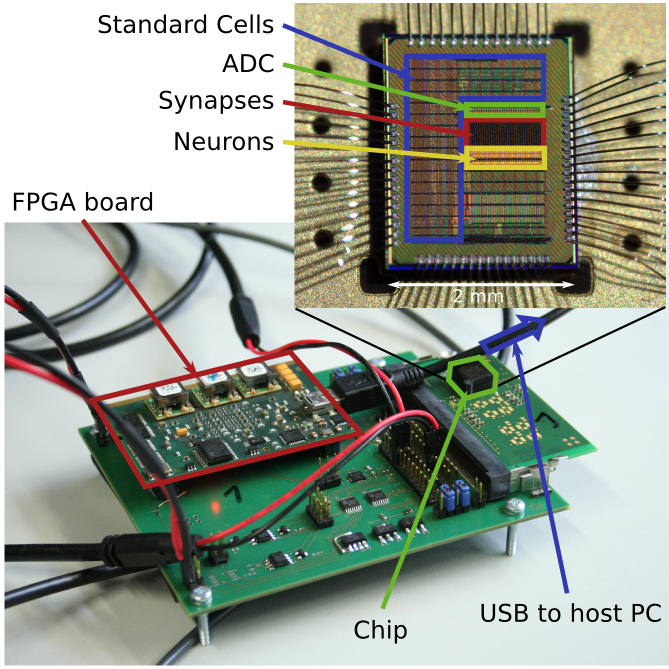
\includegraphics[width=0.4\textwidth]{pictures/Fig1.png}
    \caption{\label{fig:dlsboard} Set-Up of a \ac{HICANN-DLS} Test System (from~\citeauthor{PPU})}
\end{wrapfigure}
\\
Until now full compiler support does not exist for the \ac{PPU} because of its modified processor architecture, which was developed solely for neuromorphic hardware.
It offers a partly customized instruction set that is optimized for its applications.
\\
The \ac{HICANN-DLS} already is an experimental platform, which is used by several users, even though of \ac{PPU}-related challenges.
Applications like in-the-loop training or \ac{STDP} have been developed and mostly do not involve the \ac{PPU} .
Even when taking the effort of learning to code for the \ac{PPU}, users are constantly challenged by missing programming features such as creating parameterized functions.
This leads to repetitive code or difficulties when integrating calibration into experiment-related code.

Offering more tools for \ac{PPU} programs could reduce the effort of developing for the \ac{PPU}, while at the same time increasing capabilities of programs.
Besides allowing full high-level programming, compiler support could also offer tools like code optimization and debugging features.
At some point compiler support may also facilitate automatic code generation as a prerequisite for implementation of very high-level languages.
Users then could create plasticity rules in existing program environments from where code is translated into \ac{PPU} programs.
This creates the need for optimization of \ac{PPU} code, like those built into virtually every compiler.
\\
\\
This thesis will focus on achieving aforementioned compiler support and briefly explain the process itself.
As fundamental knowledge of both, processors and compilers, is needed along the way, the second chapter will start with a very basic introduction to both topics.
This involves basic information about the \ac{PPU}, as well as the \ac{GCC}, and should explain the basic concepts to an extend which is sufficient.
Afterwards, the process of extending the compiler is explained, followed by a presentation of results as well as first test cases.
The thesis will conclude in a resume and give an outlook to future applications and development of the compiler and the \ac{PPU}.


\chapter{Fundamentals and Applications of Computer Architectures and Compiler Design}
\label{chapter:methods}

\section{Hardware Implementation of Neural Networks}
As this thesis mainly focuses on a processor that is an essential part of the \textbf{HICANN-DLS} (High Input Count Analogue Neural Network-Digital Learning System) we will focus first on the HICANN-DLS as a whole and then look into the \textbf{PPU} (Plasticity Processing Unit) in detail while also addressing processor architecture in general.

The HICANN-DLS was built to emulate neural networks at high speeds with low power consumption.

On a very abstract level neurons in the brain resemble nodes in a network.
Neurons are interconnected through dendrites, synapses and axons which can be of different coupling strength. 
In contrast to many other systems \reference{other systems} we use neuron model that is \textbf{spike based}.
This means that a neuron is activated only for a short continuous time, called a spike, and sends out this spike through its axon to neurons that are connected via synapses.
Between those spikes the neuron is resting and not sending any signals.
Synapses can work quite differently but have in common that there is a certain weight associated to them, which we will call synaptic weight.
This is equal to a gain with which the pre-synaptic signal is either amplified or attenuated.
The signal is then passed through the dendrite of the post-synaptic neuron to the soma where all incoming signals are integrated.
If the integrated signals reach a certain threshold the neuron spikes and sends this signal to other neurons~\citep{silbernagl2009color}.

\add{bild synaptic array}

\subsection{Implementation in HICANN-DLSv2}
The HICANN-DLS system implements a simplified neural network model in analogue electronics in order to emulate neuronal networks in a biologically plausible parameter range.

At its core it has a so called \textbf{synaptic array} that connects 32 neurons which are located on a single chip to 32 different pre-synaptic inputs.
Pre-synaptic inputs are arranged along one side of the chip which is orthogonal to the arrangement of the neurons.
They enclose a 2D field which will be our synaptic array as it mainly consists of synapse circuits.
All neurons reach into the array through conductors that are organized in columns.
The pre-synaptic inputs respectively have conductors that resemble rows in the array.
At each intersection of of those conducting lines, a synapse is placed that thereby connects a neuron and a pre-synaptic input.
Overall this gives 1024 synapses that interconnect every neuron and every synapse.

A \textbf{field programmable gate array} (FPGA) is connected to all pre-synaptic inputs and feeds external spikes into the ship which can either be computed by the FPGA or routed spikes from another ship.
Along an input row the signal of one pre-synaptic input reaches all synapses that connected and is processed individually.
Each synapse holds a 6-bit wide \textbf{synaptic weight} and an internal decoder address, which both can be changed from outside.

The FPGA sends a 6-bit address whenever it sends a spike to a pre-synaptic input which then is compared by each synapse to the addresses they hold themselves.
In case the addresses match, each synapse multiplies an output signal with the weight it stores and sends the result along a column where is reaches a neuron.
All signals that are sent, are collected along a column and reach the neuron.
Inside the neurons the resulting current input is evaluated in regard to a threshold and other parameters which decide on whether the neuron is spiking or not.
If the neuron is spiking it sends an output signal to the FPGA which is responsible for spike routing in the first place.
All of this is done continuously and may not follow discrete time steps.
Along each column sits a \textbf{correlation ADC} (CADC) that converts the signal one neuron receives into digital data for analysis but can also be accessed by the PPU similar to the synaptic array.

The HICANN-DLS is also equipped with a processing unit that includes a vector extension and some memory for it to operate on.
This is the plasticity processing unit (PPU) which is also connected to the synapse array for it to read and write synaptic weights.

The will use the following naming convention throughout this thesis:
\begin{description}
    \item[Plasticity Processing Unit PPU] is the processor which is part of HICANN-DLS and mainly responsible for plasticity of synapses.
    \item[nux] refers to the complete architecture of the PPU together with its vector extension.
    \item[s2pp] is short for synaptic plasticity processor but we will use this as name of the vector extension.
\end{description}

Synapses in the synapse array are realized as small repetitive circuits that contain 8 bits of accessible information each although only 6 bits are used as weights and the spare two upper bits are used for calibration.
The synapse array can also be used in 16-bit mode for higher accuracy that combines the weights of two synapses to a 12-bit weight.
\add{figure synapse}

Digital configuration of the synapses and writing PPU programs to the memory is handled by an FPGA that has access to every interface of a HICANN-DLS chip.

\subsection{The Plasticity Processing Unit}
The PPU, which was designed by \citep{PPU}, is a custom processor, that is based on the Power Instruction Set Architecture (PowerISA), which was developed by IBM since 1990. 
Specifically the PPU uses POWER7 which is a successor of the original POWER architecture and was released in 2010 and runs at 100 MHz clock frequency.
It is a 32-bit architecture therefore registers are 32 bit wide.

It was developed to handle plasticity and as such applies different plasticity rules to synapses during or in between experiments.
This is done much faster by the PPU than by the FPGA which is important for achieving experimental speeds that are $10^{3}$ times faster than their biological counterparts.
In general the PPU is meant to handle plasticity of the synapses during experiments while the FPGA should be used to initially set up an experiment, manage spike input and record data 

The PPU is accompanied by 16 kiB of memory as well as 4 kiB of instruction cache which together is called the plasticity sub-system.
The PPU's distinct feature is its special-function unit, the s2pp vector extension (VE), that allows for Single Input Multiple Data (SIMD) operations.
The VE is only weakly coupled to the general purpose processor (GPP) of the PPU.
Both parts can operate in parallel while interaction is highly limited.

All instructions for the VE must first pass the GPP though, which detects vector instructions and passes them to the VE as it is usual for most processor extensions.
These instructions then go into a queue that holds all vector instructions where they are fetched from in order.
Going from there, the instructions shortly stay in a reservation station that is specific for each kind of operation an thus allows for little out of order operation for instructions in these reservations stations.\add{figure vector extension}
This allows for performing some arithmetic operations on a vector during the process of accessing a different vector in memory.
The result is faster processing speed as pipelining for each instruction is also supported.
The limiting factor for this though remains the vectors register file's single port for reading and writing.

Although the main limiting factor in processing speed is the memory access, both, the GPP and the VE, share the same MMU and thus any access of the GPP to vectors in memory must be handled with care as, the GPP and VE are not synchronized.
The MMU is very simple as it does not cache memory instructions and also has matching virtual and physical addresses.

For this reason one must be aware of the |sync| instruction that is a memory barrier and stops the GPP from executing instruction until all memory requests of GPP and VE are handled.
\add{code example}
This can result in up to a few hundred cycles of waiting for memory access to be finished and therefore this should only be done if necessary.
|sync| is a standard instruction of the PowerISA and further information can be found here. \add{reference}

The PPU is also able to read out spike counts and additional information through a bus which is accessible through the memory interface.
It uses the upper 16 bits of a memory address which are available because the memory is only 16 kiB large which is equivalent to 16-bit addresses.
The lower 16 bits are used since the system uses big-endian numbers.\unsure{maybe different}
A pointer to such a virtual memory address allows to read for example spike counts during an experiment.
This is done the same way for the whole chip configuration such as analog neuron parameters.

Besides the VE and the GPP, the memory bus also accessible by the FPGA .
This is needed for writing programs into the memory as well as getting results during or after experiments also allows for communication between a ``master'' FPGA and a ``slave'' PPU.

Hence the vector unit was equipped with an extra bus that connects to the mentioned synapse array.
The synapse array though is alternatively accessible through the main memory bus by setting the first bits similar to the spiking rate information.
Using this extra bus or the instructions associated with it is more comfortable and gives more structure to the program but does not increase performance of memory access.
As mentioned before, the GPP and VE share a memory bus but vector memory instructions need to pass the VE first which leads to delay that makes inserting a heavy weight memory barrier or ``syncing'' necessary at times.

Specifically the vector extension allows for either use of 8 element vectors with elements being halfword (1 halfword = 2 bytes) sized or 16 element vectors with each element byte sized
Thus every vector is 16 bytes or 128 bits long.\add{figure of vector size}
This is also the size of each vector register that is available, which are 32 in total, in contrast to 32 general purpose registers with 32 bit each.
The VE also features a vector accumulator of 128 bits width and a vector condition register which holds 3 bits for each half byte of the vector, making 96 bit in total, that determine which condition applies.

To handle the vector unit the instruction set was extended by 53 new vector instructions that partly share their opcodes with existing AltiVec instructions.
This renders no problem since the nux does not recognize AltiVec opcodes and most like is not going to in the future.
An overview of all opcodes is provided by \cite{nuxmanual}, which is recommended as accompanying literature besides this thesis.
In general these opcodes are divided into 6 groups of instructions:
\begin{description}
    \item[modulo halfword/byte instructions] apply a modulo operation after every instruction which causes wrap around in case of an overflow at the most significant bit position.
        Each instruction is provided as halfword (modulo $2^{16}$) and as byte instruction (modulo $2^{8}$).
    \item[saturation fractional halfword/byte instructions] allow for the results only to be in the range between a maximum that is equivalent to one when we see the MSB as $2^{-1}$ and the minimum is $2^{-15}$ for halfword and $2^{-7}$ for byte instructions. \todo{check with ahartel on this}
    \item[permute instructions] perform operations on vectors that handle elements of vectors only as a series of bits.
    \item[load/store instructions] move vectors between vector registers and memory or the synapse array.
\end{description}

When using these instruction one must always keep in mind that the weights of the synapses only consist of the latter 6 or 12 bits which are in a vector register and are right aligned.
As a user still wants the full functionality and also as much accuracy as possible, a vector is typically shifted left when reading from the synapse array to  align the MSB to the very left and thus right shifted when stored in the synapse array.

\add{applications of the PPU today like in-the-loop experiments and controlling
}

\section{Basics of Processor Architecture}
\label{section:processor}

Almost all contemporary processors are built using the so called von-Neumann architecture \todo{add reference}.
\todo{cite friedmann dissertation}Although the main goal of this project is to provide an alternative analogue architecture that is inspired by nature, there are advantages to classic computing which are needed for some applications.

The main advantage of digital systems over analogue, systems such as the human brain, is the ability to do numeric and logical operations at much higher speeds and precision as well as the availability of existing digital interfaces.
For this reason ``normal'' processors are responsible for handling experiment data as well as configuration of an experiment.
We will now shortly touch the basics of such processors and explain common terms.
\\
\\
\add{figure classic architecture}
In general a microprocessor can be seen as a combination of two units which are an operational section and a control section.
The control section is responsible for fetching instructions and operands, interpreting them, controlling their execution as well as reading and writing to the main memory or other buses.
The operational section on the other hand saves operands and results only as long as they are needed and performs logic or arithmetic operation on these as instructed by the control section.
Prominent parts of the operational section are the \textbf{arithmetic logic unit} (ALU) and the \textbf{register file} (RF).

The register file can be seen as short-term memory of the processor.
It consists of several repeated elements, called \textbf{registers}, that save data and have a same size which is determined by the architecture; a 32-bit architecture has 32-bit wide registers.

Typically the number and purpose of registers varies for different architectures.
Common purposes of registers are:
\begin{description}
    \item[general-purpose register GPR] These registers can be used for virtually anything and in most cases carry values that are soon to be used by the ALU. Most registers on a processor are typically GPRs.
        Any register that is not a GPR is called a \textbf{special purpose register SPR}
    \item[link register LR] This register marks the jump point of function calls. This means that after a function completes, the program jumps to the address in the link register.
    \item[condition register CR] This register's value is set by an instruction that compares one or two values in GPRs. Its value can determine a condition for some instructions if they are to be executed or not.
\end{description}        

The ALU uses values which are stored in the register file to perform the aforementioned logic or arithmetic operations and saves the results there as well.

Some architectures also have an accumulator that is often part of the ALU.
Intermediate results can be stored there because access to the accumulator is the fastest possible but holds only a single value.

It is important to note:
\begin{equation*}
    \text{speed(accumulator)} > \text{speed(register)} \gg \text{speed(memory)}
\end{equation*}
As speed is always important in computing we therefore want to rather use registers than memory and only write to memory when not enough registers are available or a task has finished.

Registers such as the accumulator can also either be accessible to a user or only accessible to subsections such as the ALU.
This is different for every processor architecture and depends on a multitude of factors:
\noindent\begin{minipage}{\textwidth}
    \vspace{1em}
    \begin{minipage}{0.4\textwidth}
\begin{itemize}
    \item available chip space
    \item maximum clock frequency
    \item instruction set complexity
\end{itemize}
\end{minipage}
    \begin{minipage}{0.6\textwidth}
\begin{itemize}
    \item available time and money for the design
    \item energy consumption
\end{itemize}
\end{minipage}
    \vspace{1em}
\end{minipage}

These factors influence one another as a complex instruction set allows for complicated arithmetic operations to be performed with a single instruction but this often results in the effective clock frequency being lower due to many micro instructions.\reference{complexity > lower clock freq}
During a single clock cycle a chip usually performs one so called \textbf{micro instruction} which is part of a \textbf{machine instruction}.
An example for an add instruction (|d = add(a,b)|) would be:
\begin{lstlisting}[caption=example of micro instructions, label=lst:microinstruction]
    1. fetch the instruction from memory
    2. decode instruction
    3. fetch first operand a
    4. fetch second operand b
    5. perform operation on operands
    6. store result
\end{lstlisting}\todo{inhaltlicher zusammenhang}
For more complex machine instructions the amount of micro instructions can be much higher, but such simple machine instructions basically set the minimum amount of micro instructions for any machine instruction.
It is obvious that the faster the clock frequency the faster micro instructions can be executed the faster the processor.
But at the same time the more complex the instruction set is the fewer machine instructions are needed overall the faster the processor.
As mentioned above this results in a trade-off between clock frequency and instruction set complexity.\reference{book}

The instruction set includes all available instructions for an ALU thus the ALU gets more complicated to design and needs more space as the instruction set gets more complex.
Because of this, one usually differs between two kinds of processors:
\begin{description}
    \item[CISC] Complex Instruction Set Computer
    \item[RISC] Reduced Instruction Set Computer
\end{description}
The latter usually is reduced to such simple instructions as |add| or |sub| and connects them to create more complex instructions.
Since the PPU is a RISC architecture we focus on RISC's key values.
Simple instructions are similar to micro instructions which were mentioned earlier, but every simple instruction has the same number of micro instructions.
RISC architectures therefore start ``pipelining'' instructions, which means starting the next machine instruction as the previous machine instruction just performed the first micro instruction in a clock cycle.
Ideally, this will increase the performance by a factor that is equal to the number of micro instructions in a machine instruction as that many machine instructions can be initiated in the same time it takes to complete a single machine instruction.
It must be noted though that the processor has to detect hazards which are data dependencies between instructions where one instruction needs the result of another.
Such instructions usually are postponed to a delay-slot and other instructions that do not cause hazards are executed instead.
This results in reordering of instructions on a processor level.
Also it takes several cycles for memory instructions to load or store data this effectively stalls the processor until the memory instruction has finished.
Therefore RISCs try to avoid memory access as much as possible and use registers instead.
Luckily a normal RISC architecture provides more registers as the ALU needs less space due to reduced complexity and also can be operated at higher clock frequencies, therefore it is perfect for simple processors that only need to do simple arithmetic as fast as possible.

Next we take a closer look at memory.
Normally the memory of a von-Neumann machine contains both, the program and data (this is contrary Harvard architectures).
The program here describes a list of instructions that are part of the instruction set.
Each instruction itself is represented as a sequence of bits in memory that resemble the following.
\add{graphic of opcode}
The first part which is called an opcode is simply a number that stands for an operation performed by the ALU.
The ALU reads this number and performs the necessary steps.
Typically this part is about 8 bits long and has an alias string such as |add| that is called a mnemonic.
The second part is the result which is of the same type as the third and forth part.
These are the argument addresses or operands of an operation and can either be a memory address or a register number as both are valid operands.
Many RISC architectures have an instruction set that consists exclusively of 3 operand instructions.
Any instructions that seem to have less than three operands are normally mapped on instructions that have three operands.
It is quite common to use more complex instructions for relatively simple instruction as this reduces the number of opcodes.
An example would be moving the contents of register 1 to register 2.
This usually maps to an or comparison between register 1 and a register that is all zeros where the result (the same as register 1) is saved in register 2.

It is important to note that in most RISC architectures if we want a memory address as operand, this is done indirectly.
A memory address can not be an operand on its own but is loaded into a different register and a different register gets to hold the data from the memory.
This is called a load instruction and its counter part would be a store instruction.
Architectures that work like that are called load/store architectures.

This means also that the amount of accessible memory is typically limited by the width of a single register
Memory is often seen as blocks and with addresses.
Because the smallest amount of information which we are interested in is a byte, each address is equivalent to one byte in memory.
Therefore the maximum amount of memory that can be used is:
\begin{equation}
    2^{n} byte \xrightarrow{\text{n = 32 bit}} 2^{32} byte \approx 4*10^{9} byte = 4 GB
\end{equation}

Normally though it is not the processor itself that keeps track of the memory.
This is usually done by a memory management unit (MMU).
It handles all memory access of the processor as it can provide a set of virtual memory addresses which itself then transforms into physical addresses.
Most modern MMUs also incorporate a cache that stores memory operations while others are handled and detects dependencies within this cache which it can resolve.
This results in faster transfer of data as two or more instructions access the same memory which then is handled in the cache.
Not all MMUs support this though and this might lead to certain problems when handling memory.
If instructions are reordered due to pipelining and dependencies on the same memory address are not detected, an instruction may write to the memory before a different one could load the previous value it needed.
For this reason exist memory barriers.
A memory barrier is an instruction that is equal to a guard in code that waits until all load and store instructions issued to the MMU are finished and then allows the code to proceed.
It therefore splits the code into instructions issued before the memory barrier and issued after the memory barrier.
Even with reordering this prohibits any instruction to be executed on the wrong side of the barrier and thereby ensures conflicting memory instructions to not interfere with one another.

Memory can be split into two popular types which are static random access memory (SRAM) and dynamic random access memory (DRAM).
The differ in how bits are set on each RAM.
SRAM uses Flip Flops to switch transistors that indicate which bit is set, while DRAM uses capacities that are charged to do so.

We already introduced many parts of a processor which need to be connected somehow.
Connections between these parts are called buses and also have a width measured in bytes.
Bus speeds are very high as they transport data in parallel such as the contents of a register.
Thus most buses should be as wide as a register of the processor.
But buses of such width need much space.
Therefore some architectures use narrower buses with fewer bits than a register and use two instructions to transfer the contents of a full register.
Systems of this sort are described as 32/16-bit architecture, which means that registers are 32 bit wide while buses are only 16 bit wide.
As the higher order bits of registers are not as often used as the lower ones this results in less performance loss than initially expected.

\subsection{Co-processors and Extensions}

RISC architectures sometimes need so called co-processors for instructions that are not included in the instruction set but are often enough needed.
An example would be multiplication which would need many cycles when split in |add| instructions but as part a co-processor can be performed in just a few cycles.
In such a case the control section recognizes the |mult| instruction and passes it to the co-processor and later on fetches the result.

This can be extended to whole units such as the ALU existing in parallel.
One example would be a floating point unit (FPU) which is nowadays standard for most processors and handles all instructions on floating point numbers.
For this the FPU has its own floating point registers (FPRs) in a separate register file on which it performs instructions and which also have parallel access to the memory.

Another kind of extensions are vector extensions that do the same as the FPU but for vectors instead of floats.
This is mostly wanted for highly parallel processes such as graphic rendering or audio and video processing \todo{reference}.
But also early supercomputers such as the Cray-1 \todo{reference} made use of vector processing to gain performance by operating on multiple values  simultaneously through a single register.
This could either be realized through a parallel architecture or more easily through pipelining the instruction on one vector over its elements.
The latter one makes sense since there are typically no dependencies between single elements in the same vector.
Nowadays many of the common architectures support vector processing.
A few examples of these are:
\begin{itemize}
    \item x86 with SSE-series and AVX
    \item IA-32 with MMX
    \item AMD K6-2 with 3DNow!
    \item PowerPC with AltiVec and SPE
\end{itemize}
As mentioned these were mostly intended for speeding up tasks like adjusting the contrast of an image.
There is also the possibility to vectorize loops in programming if there are no dependencies between loop cycles.
    

\subsubsection{AltiVec Vector Extension}
In our case we take a special interest in the AltiVec vector extension which developed by Apple, IBM and Motorola in the mid 1990's and is also known as Vector Media Extension (VMX) and Velocity Engine for the POWER architecture. 
The AltiVec extension provides the processor with a single-precision floating point and integer SIMD instruction set.
The vector register file includes 32 vector registers are each 128-bit wide. \cite{AV:registers}
These vector registers can either hold sixteen 8-bit |char|s, eight 16-bit |short|s or four 32-bit |int|s or single precision |float|s, each signed and unsigned.
Single elements of these vectors can only be accessed through memory because there is no instruction that combines scalar register with vector registers.
Except for one type of instruction that ``splats'' the value of a scalar register into all elements of the vector register.
The reason we take such an interest in this vector extension is that it resembles most characteristics of the PPU's vector extension and is already implemented in the PowerPC back-end of GCC.
There a few differences though:
\begin{addmargin}[2em]{0em}
    First the PPU's VE uses a conditonal register (CR) to perform instructions only on those elements of a vector register, that meet the condition in the corresponding part of the CR, which is specified by the user, while the AltiVec VE utilizes the CR which included in the PowerPC architecture.
    This results in not allowing selective operations on individual elements through the CR but allows for checking if all elements meet the condition in a single instruction.
    If element-wise selection is needed AltiVec offers this through vector masks.
    
    The AltiVec VE has two register on its own though, which are the VCSR and VRSAVE registers.
            The Vector Status and Control Register (VSCR) is responsible for detecting saturation in vector operations and decides which floating point mode is used.
            The Vector Save/Restore Register (VRSAVE) assists applications and operation systems by indicating for each VR if it is currently used by a process and thus must be restored in case of an interrupt.
    
    Both of these register are not available in the PPU's VE but would likely not be needed for simple arithmetic tasks as the PPU is meant to perform.
\end{addmargin}



\section{Basic Compiler Structure}
\label{section:compiler}
At its core every compiler translates a source-language into a target-language, most often it translates a high-level, human readable programming language into a machine language that consists of basic instructions that build complicated structures.
In doing so compilers may be the essential part in everyday lives of programmers everywhere.
But compilers do not exist as long as computers do and their development played a big role in making computers such an important part of everyday life as they are today.
What differs compilers from the competing concept of interpreters is the separation of compile-time and run-time.
As interpreters combine these two and translate a program as it is run, a compiler takes the time to read the source-language file completely (often several times) and only then creates the executable files which are run after the process has finished.
The advantages of this are simple:
While a compiler takes some time at first until the program can be run, the resulting executable is next to always faster and more efficient.

\begin{figure}
    
    \tcbset
    {enhanced,colframe=blue!70!black,colback=white!50!blue,colupper=red!50!black,
    fonttitle=\bfseries,nobeforeafter,center title, noparskip}
    \noindent{\begin{minipage}{\textwidth}
        \begin{minipage}[c][][c]{0.25\textwidth}
            \begin{tcolorbox}[tcbox raise base, width=\linewidth, remember as=cp, enhanced, watermark text=Compiler]
                \begin{tcolorbox}[enhanced, breakable, noparskip,opacityframe=0.0, opacityback=0.0, height=2cm, width=\linewidth]
                \end{tcolorbox}
                \begin{tcolorbox}[enhanced, breakable, noparskip,opacityframe=0.0, opacityback=0.0, height=1cm, width=\linewidth]
                \end{tcolorbox}
                \begin{tcolorbox}[enhanced, breakable, noparskip,opacityframe=0.0, opacityback=0.0, height=1.5cm, width=\linewidth]
                \end{tcolorbox}
            \end{tcolorbox}
            \begin{tikzpicture}[overlay,remember picture,line width=1mm]
                \draw[->, shorten >=-1.5mm] ($(cp.north)+(0,1)$) -- node [left] {program code} (cp.north);
                \draw[->] (cp.south) -- node [left] {machine files} ($(cp.south)+(0,-1)$);
            \end{tikzpicture}
        \end{minipage}
\end{minipage}}

    \caption{\label{fig:compiler} Schematic overview of different compiler stages.}
\end{figure}


This is due to the possibility of optimizing code during the compilation process and the chance of reading through the source file several times if this is needed (with each time the code is read being called a ``pass'').
Of course there do exist several compilers today and what matters to the user is typically the combination of the amount of time it takes to compile a program and the performance of that program.
Though a compiler is not solely involved into the processing of a programming language towards an executable program.
Figure~\ref{fig:compiler} illustrates the chain of tools that is involved into this process:
As one can see the \textbf{preprocessor} modifies the source before it is processed by the compiler and removes comments, substitutes macros and also includes other files into the source.
After the compiler is finished with its job the \textbf{assembler} takes over and translates the output of the compiler which is written in a language called assembly into actual machine code by substituting the easy-to-read string alternatives with actual opcodes.
At last the \textbf{linker} combines the resulting ``object-files'' that the assembler emitted for different source files with standard library functions that are also already compiled and other resources. 
The result is a single file that is directly executable.
The only task which is left for the \textbf{loader} is assigning a base address to the relative memory references of the ``relocatable'' file which were used until now.
The code is now fully written in machine language and ready for operation.

But since we are more interested in compilers than other components, we will take a better look at the compiler itself.
Figure~\ref{fig:compiler} shows the common separation of a compiler into front-end, back-end and the optional middle-end.
This is done to make a compiler portable, which means allowing the compiler to work for different source-languages which are implemented in the front-end and target-languages which must be specified in the back-end.
Therefore if one wants to compile two different programs e.g. one in C the other in FORTRAN, it is necessary to change the front-end but not the back-end because the machine or ``target'' stays the same.
The middle-end in this regard is not always needed but could be responsible for optimizations that are both source-independent and target-independent.
Of course the different parts of the compiler have to communicate through a language that all parts can understand or speak.
Such a language is called intermediate representation (IR) and also used during different phases of the compilation process.
It may differ in its form but always stays a representation of the original program code.

The different phases of a compilation process are illustrated to the far right of figure~\ref{fig:compiler}.
There is no middle-end included into this scheme as it is not a mandatory part of the compiler and would only be responsible for optimizations.
But we will take a short look at the other phases:
First the source code is fed into the \textbf{scanner} that performs lexical analysis, which is combining sequences of characters to symbols of something called tokens that get associated with an attribute such as ``number'' or ``plus-sign'' and the symbol.
Next the \textbf{parser} takes the sequence of tokens and builds a syntax tree that represents the structure of a program and is extended by the \textbf{semantic analyzer} which adds known attributes at compile-time like ``integer'' or ``array of integers'' and checks if the resulting combinations of attributes are valid.
This already is the first form of IR.
The \textbf{source code optimizer} which is the last phase of the front-end takes the syntax tree and takes the first shoot at optimizing the code.
Typically only light optimization is possible at this point such as pre-computing simple arithmetic instructions and different kinds of optimization exist.
After the source code optimizer is done the syntax tree is converted to intermediate representation in order to be passed to the back-end.

The \textbf{code generator} takes this IR and translates it to machine code that fits the target - typically this is assembly.
At last the \textbf{target code optimizer} tries to apply target-specific optimization until the target code can be emitted.

During these phases the compiler also generates a symbol and literal table.
A symbol table is as the name states an overview of all symbols that are used in the program, it contains the symbols name and the attribute of the semantic analyzer.
A literal table in contrast holds constants and strings and makes them available globally by reference, as does the symbol table.
This information is used by the code generator and various optimization processes.

\subsection{Back-End and Code Generation}
We now want to focus a little more on the last two phases of a compiler, which are also part of the back-end.
We already stated that the back-end is responsible for code generation and target optimization and since we will keep focus on the back-end later on, we need to get used to a few other terms that are common when talking about compiler back-ends.

Usually the processes of code generation and target optimization are entangled as optimization can take place at different phases of code generation.
Thus we first take a look at code generation in the back-end.

As we learned already, the source program reaches the back-end in form of IR.
Often the IR is already linearized and thereby again in a form that can be seen as sequence of instructions.
Because of this the IR may also be referred to as Intermediate Code.
The process of generating actual machine code from this is again split into different phases:
\begin{itemize}
    \item instruction selection
    \item instruction scheduling
    \item register allocation
\end{itemize}

At first the back-end recognizes sets of instructions in intermediate code that can be expressed as an equivalent machine instruction.
Depending on the complexity of the instruction set a single machine instruction can combine several IR instructions.
This may involve additional information that the front-end aggregated and added to the IR as attributes single machine instruction can combine several IR instructions.
At the end of this is a compiler typically emits a sequence of assembly instructions which we will explain later on.
In order to fulfill this task the compiler needs the specifications of the target it compiles for.
This is called a target description and can contain things like specifications of the register-set, restrictions and alignment in memory and availability of extensions and functionalities.
The compiler also needs knowledge of the instruction set of a target sometimes referred to as the ISA which is in essence a list of instructions which are available and also their functionality.
The compiler picks instructions according to their functionality from this list and substitutes the IR with this.
Ideally a back-end thus could support different back-ends just by exchanging the machine description and the ISA as the basic methods of generating code are the same for most targets.

After the IR is converted into machine instructions the back-end now rearranges the sequence of instruction.
This needs to be done as different instructions take different amounts of time to be executed.
If a subsequent instruction depends on the result of a previous instruction the compiler now has two alternative approaches to solve this.
First it can simply stall the programs execution as long as the instruction is executed and feed the next instruction into the processor only when the dependency is solved.
This means that the compiler adds |nop|s before every instruction that needs to wait for an operand as |nop| tells the processor to wait until the previous instruction has finished.
For critical memory usage the compiler can also insert |sync|s as memory barriers before hazardous memory instructions.
Alternatively it can stall only the instruction which depends on the result which is currently computed but perform instructions that do not depend on the result in the mean time.
By doing so the scheduler increases performance noticeably and thus can partly be seen as part of the optimization process.
On RISC architectures this is especially important as load and store instructions can take a few hundred times more clock cycles than normal register instructions and pipelining depends mainly on the instruction sequence.
Thus the scheduler is also involved parallelization of code.
As a result of this a compiler would usually accumulate all load instructions at he beginning of a procedure and start computing on registers that already have a value while the others are still loaded.
This is done vice versa at the end of a procedure for storing the results in memory.
This process of course needs the compiler to know the amount of time it takes for an instruction to be executed and works hand in hand with hazard detection on processor level.

At last he compiler handles register allocation which also includes memory handling.
Typically the previous processes expect an ideal target machine which provides and endless amount of registers.
As in reality the processor only has $k$ registers the register allocator reduces the number of ``virtual registers'' or ``pseudoregisters'' that are requested to the available number of ``hard registers'' $k$.
For this to be possible the compiler decides whether a value can live throughout a procedure in a register or must be placed into memory because there are not enough registers available.
This results in the allocator adding load and store instructions to the machine code in order to temporarily save those registers in memory which is called ``spilling''.
It is obvious that this can hurt performance and therefore the compiler tries to keep spilling of registers to a minimum and also insert spill code at places where it delays other instructions as little as possible.
At he end of register allocation the compiler assigns hard registers to the virtual registers which are now only $k$ at a time.

During and after code generation the compiler also applies optimizations to the machine code.
Any optimization to the code though must take three things into consideration, which are safety, profitability and risk/effort.
The first thing which always must be fulfilled, is safety.
Only if the compiler can guarantee that an optimization does not change the result of the transformed code compared to the original code it may use this optimization!
Only if this applies the compiler may check for the profit of an optimization which most often is a gain in performance but could also be the size of the program.
At last the effort or time it takes for the compiler to perform this optimization and the risk of generating actually bad or ineffective code should be taken into account as well.
If optimization passes these three aspects it may be applied to the code.
In the end there exist some simple optimizations that always pass this test like the deletion of unnecessary actions or unreachable code, e.g. functions that are never called.
Another example would be the reordering of code like the scheduler did before or the elimination of redundant code, which applies if the same value is computed at different points and thus the first result simply can be saved in a register.
If a compiler knows the specific costs of instructions, it can also try to substitute general instruction with more specialized but faster instructions, like substituting a multiplication with 2 by shifting a value one position to the left.
There exist many more ways of optimization but we only want to explain one more kind of optimization which is called peephole optimization.

In peephole optimization the compiler only looks at a small amount of code through a ``peephole'' and tries to find a substitution for this specific sequence of instructions.
These substitutions must be specified by hand and are highly target-dependent in contrast to the optimizations which were mentioned before that are target-independent.
If the sequence can be substituted the peephole optimizer does so, otherwise the peephole is moved one step further and the new sequence is evaluated.

\subsection{Assembly Basics}
\label{section:asm}
Assembly (|asm|) was mentioned a few times in this thesis already and we need to know at least a few basic assembly instructions that will help us later on to understand resulting machine code.
Assembly is usually the lowest level of representation of a program that still is human-readable.
Assembly code is basically equivalent to machine code and therefore by many seen as such though assembly code needs to be assembled by the assembler first.
Assembly instructions all follow a certain scheme which is:
\begin{lstlisting}
    add r1, 0x3000, 5
    mnemonic operand/result operand operand
\end{lstlisting}
For RISC architectures instructions typically consist of 3 operands because operations are usually between registers only (except for load/store a.k.a. memory instructions).
The mnemonic in most cases is a named after the first letters of the instructions full name, which is emphasized in the following table.
The operand can be of three different types which are all shown above.
They either represent a specific register (r1 = register 1), a memory address (0x3000 = the value at memory location 0x3000) or an immediate value (5 = the integer 5).
Register operands can also have an indirect use, which means that that content of the register is taken into account.
I.e. a memory address can be saved to the register and an operation uses the value at the memory location which the register refers to.

\begin{tabular}{l l p{9cm}}
    mnemonic & operands & description \\
    \hline
    |add| & |RT, RA, RB| & \textbf{add} |RB| to |RA| and store the result in |RT| \\
    |addi| & |RT, RA, SI| & \textbf{add} |SI| to |RA| and store the result in |RT| \\
    |addis| & |RT, RA, SI| & \textbf{add} |SI| \textbf{s}hifted left by 16 bit to |RA| and store the result in |RT| \\
    |and| & |RA, RS, RB| & |RS| and |RB| are \textbf{and}ed and the result is stored in |RT| \\
    |b| & |target_addr| & \textbf{b}ranch to the code at |target_addr|\\
    |ble| & |BF, target_addr| & \textbf{b}ranch to the code at |target_addr| if |BF| is \textbf{l}ess or \textbf{e}qual \\
    |blr| & & \textbf{b}ranch to the code at address in the \textbf{l}inker \textbf{r}egister \\
    |cmp| & |BF, L, RA, RB| & |RA| and |RB| are \textbf{c}o\textbf{mp}ared and the result (|gt,lt,eq|) is stored in |BF|, |L| depicts if 32-bit or 64-bit are compared \\
    |cmplwi| & |BF, RA, SI| & |RA| \textbf{c}o\textbf{mp}ared \textbf{l}ogically \textbf{w}ordwise with \textbf{i}mmediate |SI| and the result is stored in |BF|\\
    |and| & |RA, RS, RB| & |RS| and |RB| are \textbf{and}ed and the result is stored in |RT| \\
    |eieio| & & |RS| and |RB| are \textbf{and}ed and the result is stored in |RT| EDITTHIS\\
    |isync| & & |RS| and |RB| are \textbf{and}ed and the result is stored in |RT| EDITTHIS\\
    |la| & |RT, D(RA)| & \textbf{l}oad \textbf{a}ggregate |D + RA| into |RT|\\
    |li| & |RT, SI| & \textbf{l}oad \textbf{i}mmediate value |SI| into |RT|\\
    |lis| & |RT, SI| & \textbf{l}oad \textbf{i}mmediate value |SI| \textbf{s}hifted left by 16 bit into |RT|\\
    |lbz| & |RT, D(RA)| & \textbf{l}oad \textbf{b}yte at address |D+RA| into |RT|, fill the other bits with \textbf{z}eros \\
    |lwz| & |RT, D(RA)| & \textbf{l}oad \textbf{w}ord at address |D+RA| into |RT|, fill the other bits with \textbf{z}eros \\
    |mflr| & |RT| & \textbf{m}ove \textbf{f}rom \textbf{l}inker \textbf{r}egister to |RT|\\
    |mr| & |RT, RA| & \textbf{m}ove \textbf{r}egister |RA| to |RT| \\
    |nop| & & halts execution until the previous instructions are finished EDITHIS\\
    |rlwinm| & |RA, RS, SH, MB, ME| & \textbf{r}otate \textbf{l}eft \textbf{w}ord in |RS| by \textbf{i}mmediate |SH| bits then a\textbf{n}d with \textbf{m}ask which is 1 from |MB+32| to |ME+32| and 0 else, store to |RA|\\
    |stw| & |RS, D(RA)| & \textbf{st}ore \textbf{w}ord from |RS| to address |D+RA|\\
    |stwu| & |RS, D(RA)| & \textbf{st}ore \textbf{w}ord from |RS| to address |D+RA| and \textbf{u}pdate RA to |D+RA|\\
    |sync| & & halts execution until the memory controller is finished EDITTHIS\\
\end{tabular}
\add{caption and reference to PPC book and asm website correct the table}

Obviously the mnemonics follow a certain pattern that has letters which can be interchanged to alter the meaning of the mnemonic, some of these characters are:
\begin{description}
    \lstitem{i} indicates that the instructions uses an immediate value
    \lstitem{b} stands for byte and references the size of the operand
    \lstitem{h} stands for halfword and references the size of the operand
    \lstitem{w} stands for word and references the size of the operand
    \lstitem{s} indicates that one of the operands is shifted
    \lstitem{g, ge, l, le, e} stand for greater, greater or equal, less, less or equal and equal which is the possible content of the conditional register
\end{description}

There are also special operands which might occur in |asm| which behave like pointers:
\begin{description}
    \lstitem{@l(C)} is equivalent to the lower order 16 bits of of |C| in the symbol table
    \lstitem{@ha(C)} is equivalent to the higher order 16 bits of of |C| in the symbol table and minds the sign extension
\end{description}

Additionally there exist markers which are intended for debugging:
\begin{description}
        \lstitem{.loc # # #} marks a line of code (file, line, column) in the source file
        \lstitem{.LVL} is a local label which can be discarded
        \lstitem{.LFB} marks the begin of a function
        \lstitem{.LFE} marks the end of a function
        \lstitem{.LC0} is a constant of the literals table at position |0|
\end{description}

\add{all these tables in the appendix}

We want to spend just a little more time on assembly as it is useful to know how to program in assembly while using C.
This is done by the following scheme:
\begin{lstlisting}
asm volatile (  "add %0, %1, %2"
                : "=r" (dst)
                : "r" (src1), "r" (src2):);
\end{lstlisting}

The line of code above tells the compiler to generate the instruction |add| in assembly which is followed by three operands.
The number |n| in |%n| indicates that the operand is specified by the |n+1|th description of an operand that follows.
The description that follows after |:| describes the output operands.
|"=r"| means that the output is to be stored in a register (letter |r| for register operand) and that the register is to be written (|=| this is called constraint).
The variable in parentheses must be declared before its occurrence and of matching type (|float| would not be allowed in this case).
The following description is that of the input operands and those must not be written!
|r| again stands for a register operand and the variable is in parentheses, the arguments are separated by commas.
After the third |:| follow clobbered (=temporarily used) registers which would also be in quotes, but these are optional arguments.
|volatile| means that the compiler must not delete the following instructions due to optimization.

As a special command |asm (:::memory);| would indicate a memory barrier to the compiler, ergo the machine instructions previous to this line and the one following may not be interchanged.

\subsection{Intrinsics}
Something that will also occur quite often later in this thesis are intrinsics.
Intrinsics are sometimes also called built-in functions and resemble an intermediate form of |asm| and a high-level programming language.
This means that by calling an intrinsic function, we tell the compiler to use a certain machine instruction that typically shares its name with the intrinsic.
What differs an intrinsic from |asm()| is that we do not need to specify constraints or registers classes but only need to keep an eye on the type of arguments.
One could easily mistake them for normal functions of library but they are directly integrated into the back-end of a compiler and thus independent of the programming language.
In order to implement intrinsics into a back-end the compiler need a certain knowledge of what the |asm| instruction does and what kind of operands it needs.

A typical field of application for intrinsics would be vectorization and parallelization of code through processor extensions.
Sometimes this is the sole option of using the machine instructions associated with them.

\subsection{GNU Compiler Collection}
The GNU Compiler Collection (GCC) is a compiler suite that supports different programming languages and targets.
Though normally it is seen as a build of GCC supports a variety of front-ends while it was built for a specific target.
This target in most cases is the processor architecture on which the user runs the compiler.
But GCC also supports the idea of a cross-compiler which is the concept of compiling code on one machine but running the code on a different machine that is also based on a different architecture.
One must though build a version of GCC locally for every back-end one wants to compile code for.
This is realized through a modular structure which follows the idea of a front-end, middle-end and back-end as it was described in section \ref{section:compiler} although some information that belongs to a back-end is also needed at the front-end, hence the compiler is built back-end specific but supports a wide variety of back-ends to choose from.

GCC itself is programmed in C++ and part of the GNU project of the Free Software Foundation.
It is wide-spread and one of the most popular compilers especially among academic institutions and small scale developers.
Every major UNIX distribution and many minor ones include GCC as a standard compiler.\cite{definitveGCCGuide:introduction}
As an open source project there is a constant development to the compiler and there exist many threads that support known bugs.

There is one major competitor though which stands besides GCC as an open source compiler suite which is Clang that is part of the LLVM (low level virtual machine).
Both support running the same source code on multiple machines while LLVM actually runs intermediate code rather than actual machine code and uses GCC to generate this intermediate code for some front-ends.
However while one can argue in favor for either one, GCC seems a little better suited for our application. \todo{reference LLVM vs. GCC on ARM, LLVM vs. Gcc in EISC}
These results have to be viewed with care, as they are based on different processor architectures but it seems like both compilers provide similar performance.
Ultimately it is the personal preference of the programmer that decides which compiler one is more comfortable with and often enough he chooses that compiler.
In our case I have chosen GCC over LLVM for two main reasons.
One is that after all GCC follows more the traditional concept of a compiler that generates machine code at the end and also I was far more familiar with GCC than with LLVM when this decision had to be made.
The other is that GCC support existed to a minimum before I started this thesis and thus there was a point to start from.
This topic will be referred to later on in the discussion but for now a short motivation seems to be sufficient.

By now GCC is a stable release version of 6.3 with version 7 in the works but we will use an older version which is used internally at the BrainScaleS project which is version 4.9.2.
Additionally we will use binutils 2.25 which was patched by Simon Friedmann and since includes the opcodes and mnemonics which are supported by the nux.
A complete specification of the libraries used and a handy script that builds a cross-compiler for the nux on PowerPC systems can be found there as well.

We take a special interest in the PowerPC back-end of GCC which is called rs/6000 for IBMs RISC system/6000 architecture that is equivalent to POWER.
According to GCCs Internals manual \cite{GCCint}, which we will refer to as the sole source of information in this regard, the back-end of GCC has the following structure:

Each architecture has a directory with its respective name in gcc/config e.g. gcc/config/rs6000 that contains a minimum amount of files.
These are the machine description rs6000.md which is an overview of machine instructions with additional information to each instruction and the header files rs6000.h and rs6000-protos.h and source file rs6000.c that handle the target description through macros and functions.
Every back-end needs these files in the GCC source and the final back-end is build from these files through the macros and functions just mentioned.
To notice a back-end in the first place the back-ends directory -here "rs6000"- must be added to the file config.gcc which also includes a list of all files in the aforementioned directory.
Most back-ends include additional files which makes a back-ends complex structure clearer but these are not mandatory and we will address these later.

Instead we address one of the most important functions which unfortunately is also one of the least documented though most complicated ones.
The function/process is called ``reload'' and is used as part of the register allocation process. \cite{GCCwiki:reload}
Specifically reload is meant to do register spilling but over almost 25 years that GCC existed until 4.9.2 it became more and more complex and basically does everything associated with register allocation (mainly moving the contents of different registers and memory around, and finding the right registers in the first place).
Over the years it thus became one of the main sources of errors when constructing a back-end and was meant to be replaced several times.
As of now reload is being replaced by LRA (local register allocator) but GCC 4.9.2 is not impacted by this therefore we are stuck with reload indefinitely.

To address possible errors in reload later on we now get to know one form of IR in GCC that is Register Transfer Language (RTL).

\subsubsection{Register Transfer Language Basics}
RTL, which is not to be mixed up with Register Transfer Level, is a form of IR the back-end uses to generate machine code.
Usually GCC uses the IR GIMPLE which looks like stripped down C code with 3 argument expressions, temporary variables and |goto| control structures.
The back-end transforms this into a less readable IR that inherits GIMPLEs structure but brings it to a machine instruction level.
It is inspired by Lisp lists and thus we will need to take a look at those at last in before we take on the task of extending a GCC back-end.

We do so in looking at one of the most fundamental RTL statements first while explaining the each part at a time.

\begin{lstlisting}
(define_insn "add<mode>3"
  [(set (match_operand:VI2 0 "register_operand" "=v")
        (plus:VI2 (match_operand:VI2 1 "register_operand" "v")
		  (match_operand:VI2 2 "register_operand" "v")))]
  "<VI_unit>"
  "vaddu<VI_char>m %0,%1,%2"
  [(set_attr "type" "vecsimple")])

(define_insn "*altivec_addv4sf3"
  [(set (match_operand:V4SF 0 "register_operand" "=v")
        (plus:V4SF (match_operand:V4SF 1 "register_operand" "v")
		   (match_operand:V4SF 2 "register_operand" "v")))]
  "VECTOR_UNIT_ALTIVEC_P (V4SFmode)"
  "vaddfp %0,%1,%2"
  [(set_attr "type" "vecfloat")])
\end{lstlisting}

There exist manuals to basically everything which is written here and the more extensive manual will be referenced at he end of each paragraph.

|define_insn| is an RTL expression that generates an RTL equivalent to a machine instruction.
One such instruction is called an insn (short for instruction) hand has several properties like a name, an RTL template, a condition template, an output template and attributes. \cite{GCCint:defineinsn}
The name in this case is |add<mode>3| (|3| for three operands) where |<mode>| is to replaced by a set of values that describe a modes. \cite{GCCint:stdnames}
A mode is the form of an operand and can be something like |si| for single integer, |qi| for quarter integer (quarter the bits of a single integer), |sf| for single float or |v16qi| for a vector of 16 elements which are quarter integers each. \cite{GCCint:modes}
There are many more modes that follow the same scheme.
In this case we do not specify the mode explicitly but use an iterator that creates a |define_insn| for every valid mode we specify. \cite{GCCint:iterator}
The second |define_insn| shows this with a specific mode.

Next follows the RTL template which is in square brackets.
All RTL templates need a side effect expression as a base which describes what happens to the operands that follow.
In our case |set| means that the value which is specified by the second expression is stored into the place specified by the first expression. \cite{GCCint:sideeffect}
The first expression that follows is a specified operand.
|match_operand| tells the compiler that what follows is a new operand.
|VI2| belongs to the mode iterator we saw earlier and is to be substituted by the equivalent mode to <mode> in caps, which can be seen for the following |define_insn|.
All modes |VI2| are to be substituted by the same real mode.
After the mode comes the index of an operand which starts at 0 for every |define_insn|.
The following string describes a predicate which tells the compiler more about the operand and which constraints it must fulfill.
Operands typically end in |_operand| and a single predicate is meant to group several different operand types.
In this case any register would be a valid operand. \cite{GCCint:predicates}
The next string specifies the operands further and is meant to fine tune the predicate.
It is called a constraint and matches the description which was taken in section \ref{section:asm}.
|=| again means that the register must be writable and |v| stands for an AltiVec vector register.\cite{GCCint:constraints}
This pattern is repeated for every operand and only changes slightly.
Though the second expression of the |set| side effect has an additional pair of parentheses because of the |plus| statement.
This is an arithmetic expression and tells the compiler that the following operands are part of an operation that results in a new value.
It is also succeeded by a mode that specifies the mode of the result.\cite{GCCint:arith}

The RTL template is matched by the compiler against the RTL it generated from GIMPLE and if the template matches the RTL is substituted by the output template that follows.

After the RTL template is finished, the condition specifies if the insn may be used.
It is a C expression an must render |true| in order to allow the matching RTL pattern to be applied.
In this case the condition is also depending on the mode iterator which substitutes |<VI_unit>| for equivalent code to that of the next |define_insn| with a matching mode. \cite{GCCint:defineinsn}

The output template is usually is similar to the |asm| template from |asm|.
The string contains the mnemonic of a machine instruction and the operands which are numbered according to the indexes of the RTL template.
Again this is depending on the mode iterator and |<VI_char>| will be substituted by a character that belongs to a machine mode. \cite{GCCint:defineinsn}

At last the insn is completed by its attributes which hold further information about the insn that is used by the compiler internally like which effect an insn has on certain register etc..
We are less interested in this, as attributes are optional and we do not add attributes to the back-end. \cite{GCCint:attributes}


The attentive reader might have noticed that only RTL template is written in RTL.
This is true but still do insn patterns belong into this section.
The RTL not only is the most important part of an insn but we will hardly see RTL outside from RTL templates.
Still should RTL be mentioned in its other form here as it is used for debugging purposes.

RTL can be split into two phases which are non-strict RTL and strict RTL.
Non-strict occurs only before |reload| and is very deliberate in specifying its operands.
Operands usually are virtual registers that have a unique number.
|match_operand| then is replaced by |(reg:SI 1)| which tells the compiler the type of operand, the mode and the register number.\cite{GCCint:regsnmem}

Strict RTL has passed |reload| and no longer contains virtual registers but only references existing hard registers or memory.

An example of non-strict RTL and strict RTL of the same code can be seen in figure \add{examples of RTL code}

\add{
MMU ?= memory controller
PPC must handle syncing in compiler when I/O is added
explain stack and frame pointer
PPU instruction set
}


\chapter{Extending the \ac{GCC} Back-End}
\label{chapter:extbackend}
The previous chapter dealt with processors, the \ac{PPU}, compilers and \ac{GCC}, which was preparation for this chapter.
This chapter will now emphasize on the task of extending the \ac{GCC} back-end.
There is a number of files, which will be systematically edited and referenced as they are important parts of the \ac{rs/6000} back-end and are changed in the process of extending the back-end. 
\begin{description}
    \item[rs6000.md] is the machine description of the back-end in general and contains insn definitions for all scalar functions
    \item[rs6000.h] is a header file which contains macros and declarations for registers
    \item[rs6000.c] is the source file which implements the back-end's functions
    \item[rs6000.opt] lists the options and flags for the target
    \item[rs6000-builtins.def] contains the definitions of intrinsics
    \item[rs6000-cpus.def] lists sub-targets that belong to the \ac{rs/6000} family
    \item[rs6000-c.c] links built-ins and overloaded built-ins
    \item[rs6000-opts.h] contains a set of enumerations that represent option values for the back-end
    \item[rs6000-protos.h] makes functions in |rs6000.c| globally available
    \item[rs6000-tables.opt] lists values to a processor enumeration
    \item[driver-rs6000.c] a collection of driver details for different targets
    \item[ppc-asm.h] sets macros for the use of |asm|
    \item[s2pp.md] is a new machine description of \ac{s2pp} and contains insn definitions
    \item[s2pp.h] is the header file that defines aliases for built-ins
    \item[constraints.md] contains definitions of constraints
    \item[predicates.md] contains definitions of predicates
    \item[vector.md] defines general vector insns
    \item[sysv4.h] initializes a variety of option flags and sets default values
    \item[t-fprules] sets soft-float as default for certain targets
\end{description}

It is recommended to have chapter 5 of the \textbf{nux manual}~\citep[ch.~5]{nuxmanual} at hand, as it contains an overview of existing \ac{s2pp} vector instructions.

Before extending the \ac{GCC} back-end a few things must be stated:

Due to the limited documentation of the back-end itself, one must rely on comments in code and the \textbf{\ac{GCC} internals manual}~\citep{GCCint} 
As a full implementation for a vector extension already exists, the AltiVec extension should be used as a guideline for a new extensions~\cite{AltiVec}. 
Still, it should be avoided to change exiting code as much as possible.
Code is often referred to from different places in the back-end and modifying existing code can therefore easily lead to compiler errors.
Especially since the back-end is not extended completely right away but rather step by step.
This applies particularly to functions that are implemented for AltiVec only.
It is recommended to rather duplicate functions and distinguish them, before they are called.
This will make it easier to find bugs, as usually the function that generates an error is indicated in the error message.
Also, there do exist enough differences between these two vector extensions, that combining functions would not save work.

It will therefore occasionally be pointed out when functions or other code can be inherited from AltiVec and which modifications are needed.

\section{Adding the s2pp Option Flag and nux Target}
Extending the rs6000 back-end starts by adding the |nux| processor to the list of targets and also including mandatory flags with this.
Ideally the user only has to add the flag |-mcpu=nux| when compiling, in order to produce machine code for the nux.
The flags which have to be set when using the nux are:
\begin{description}
        \lstitem{-msdata=none}
        disables the use of a \textbf{small data section} which is like a data section but has a register constantly referring to it and thus has faster access than the normal data section. Globals, statics and small variables that are often used are preferably stored there. It is turned off because the base pointer is not initialized by the linker and the effect of a small data section would likely be small for the \ac{PPU}~\cite{nuxmanual, ibmsda, websda}.
        \lstitem{-mstrict-align}
        aligns all variables in memory which means that a variable always starts at a memory address which is a multiple of its size. E.g. a vector has always an address that is dividable by 16 bytes or 128 bits. Memory management is far easier for aligned variables.
        \lstitem{-msoft-float}
        tells the compiler that there is no FPU and all floating point operations have to simulated by software.
        \lstitem{-mno-relocatable}
        states that the program code has a fixed memory address that may not be altered. Relocatable code is not needed as the \ac{PPU} runs only one program that is loaded into memory and uses no environment on top.
\end{description}

But first there should be an \textbf{option flag} that activates nux' \ac{VE} like |-maltivec| does for the AltiVec \ac{VE}.
The name for this new option flag will be |-ms2pp| and it will define an option mask along with it.
In |rs6000.opt| and we simply need to add:
\begin{lstlisting}
ms2pp
Target Report Mask(S2PP) Var(rs6000_isa_flags)
Use s2pp instructions
\end{lstlisting}
This adds |ms2pp| to the list of option flags and the next lines defines a macro, that is associated with it.
|Target| means that the option is target specific, therefore only certain architectures support the option flag.
|Report| means that the option is printed when |-fverbose-asm| is is set.
|Mask(S2PP)| initializes a bitmask, that is available through |OPTION_MASK_S2PP|.
That macro is attached to |rs6000_isa_flags|, which is specified by |Var|.
It simultaneously specifies a macro |TARGET_S2PP| that is set to |1|~\citep[ch.~8]{GCCint}.

This needs also specification of 
\begin{lstlisting}
#define MASK_S2PP OPTION_MASK_S2PP
\end{lstlisting}
in |rs6000.h| as macros with |MASK_| are a standard from earlier versions of \ac{GCC}.

Although this option flag shall later enable \ac{s2pp} support, it needs the aforementioned flags as well, to compile nux programs.
For this reason exists a processor type which combines those flags.
There exist several lists that contain available targets and nux shall be included.
First an inline assembly (see section~\ref{section:asm}) flag is created, which tells the assembler which system architecture is used.
As nux is based on POWER7, one can copy the flag |-mpower7| in |driver-rs6000.def|:
    \begin{lstlisting}[caption=\tt rs6000.h]
    #define ASM_CPU_SPEC \
        ...
        %{mcpu=power7: %(asm_cpu_power7)} \
        ...
        %{mcpu=nux: %(asm_cpu_power7)} \
        ...
    \end{lstlisting}
    \begin{lstlisting}[caption=\tt driver-rs6000.c]
    static const struct asm_name asm_names[] = {
        ...
        { "power7",   "%(asm_cpu_power7)" },
        ...
        { "nux",  "%(asm_cpu_power7)" },
        ...
    \end{lstlisting}
This will set the assembler |-mpower7| when using |-mcpu=nux|.

The nux target should also be recognized by preceding phases of the compiler and set option flags accordingly.
These options flags can be set in |rs6000-cpus.def|.

\begin{lstlisting}
...
RS6000_CPU ("nux", PROCESSOR_POWER7, MASK_SOFT_FLOAT | MASK_S2PP | MASK_STRICT_ALIGN | !MASK_RELOCATABLE)
\end{lstlisting}

This uses the macro |RS6000_CPU (NAME, CPU, FLAGS)| and adds |nux| to the |processor_target_table[]|.
Since option flags usually set masks, one can set the respective masks directly.
The masks will tell the compiler that the processor is a POWER7 architecture and uses |soft-float|, |strict-align| and |no-relocatable|(negated relocatable) as well as the new s2pp mask.

It is not possible, to set the |-msdata=none| flag before since the |-msdata| flag is initialized differently.
Also since it is not simply set ``on'' or ``off'' but accepts several values, it is handled in |sysv4.h|.
|rs6000_sdata| will be set according to the string that follows |-msdata=|.
\begin{lstlisting}
#define SUBTARGET_OVERRIDE_OPTIONS                          \
...
  if (rs6000_sdata_name)                                    \
     {                                                      \
       if (!strcmp (rs6000_sdata_name, "none"))             \
     rs6000_sdata = SDATA_NONE;                             \
     ...
       else                                                 \
     error ("bad value for -msdata=%s", rs6000_sdata_name); \
     }                                                      \
  else if (OPTION_MASK_S2PP                                 \
          && OPTION_MASK_SOFT_FLOAT                         \
          && OPTION_MASK_STRICT_ALIGN                       \
          && !OPTION_MASK_RELOCATABLE)                      \
     {                                                      \
     rs6000_sdata = SDATA_NONE;                             \
     rs6000_sdata_name = "none";                            \
     }                                                      \
  else if (DEFAULT_ABI == ABI_V4)                           \
...
)\todo{looose this!!!!!!!!!!!!!!!!!!!!!!}
\end{lstlisting}

It is not possible to detect in this file, if the nux flag is set.
It therefore needs a little workaround that helps setting the value of |rs6000_sdata|.
If |-msdata| is not set, i.e. only |-mcpu=nux| is set, the compiler will use |if|-clauses that determine which value is assigned to |rs6000_sdata|.
It is possible, to add a case that checks for all flags, that are set by |-mcpu=nux| and set |rs6000_sdata| to |SDATA_NONE| if this applies.
Hence the target options will set |rs6000_sdata| to |SDATA_NONE|.

There exists a case for which this condition applies even when |nux| is not set as target, but all flags are set by hand.
If one chooses an explicit value for |-msdata|, this case does not apply though and the value of |-msdata| is set accordingly.

This is not an ideal solution, but a trade-off with as few side effects as possible.
\\
\\
Already this would allow for the use of |-mcpu=nux| as target and |-ms2pp| as option flag.
But since the flags we used are basically mandatory to the \ac{s2pp} extension, the compiler should check for these flags before starting compilation.
First though for each flag needs a macro, which the back-end can identify.
This is done in |rs6000-c.c| where \textbf{global macros} can be defined:
\begin{lstlisting}
rs6000_target_modify_macros (bool define_p, HOST_WIDE_INT flags,
                 HOST_WIDE_INT bu_mask)
{...
  if ((flags & OPTION_MASK_S2PP) != 0)
   rs6000_define_or_undefine_macro (define_p, "__S2PP__");
  if ((flags & OPTION_MASK_STRICT_ALIGN) != 0)
   rs6000_define_or_undefine_macro (define_p, "_STRICT_ALIGN");
  if ((flags & OPTION_MASK_RELOCATABLE) != 0)
   rs6000_define_or_undefine_macro (define_p, "_RELOCATABLE");
  if (rs6000_sdata != SDATA_NONE)
   rs6000_define_or_undefine_macro (define_p, "_SDATA");
   ...}
\end{lstlisting}

If |flags| and the respective option masks are set, |rs6000_define_or_undefine_macro| will define a macro that is specified by the second argument.
Whether a macro is defined or undefined depends on the boolean |define_p|, which is set by the compiler.

These new macros can be used to check if flags are set.
This needs a new file, that will also be needed later on as the \textbf{\ac{s2pp} header file}.
|s2pp,h| must be indexed in |gcc/config.gcc| under |extra_headers|.
\begin{lstlisting}
...
powerpc*-*-*)
    cpu_type=rs6000
    extra_headers="ppc-asm.h altivec.h spe.h ppu_intrinsics.h paired.h spu2vmx.h vec_types.h si2vmx.h htmintrin.h htmxlintrin.h s2pp.h"
    need_64bit_hwint=yes
    case x$with_cpu in
    xpowerpc64|xdefault64|x6[23]0|x970|xG5|xpower[345678]|xpower6x|xrs64a|xcell|xa2|xe500mc64|xe5500|Xe6500)
    cpu_is_64bit=yes
    ;;
    esac
    extra_options="${extra_options} g.opt fused-madd.opt rs6000/rs6000-tables.opt"
    ;;
...
\end{lstlisting}
This is done, so \ac{GCC} invokes the header file, as it is not referenced elsewhere.

|s2pp.h| can now be used to check the compiler flags.
\begin{lstlisting}
/* _S2PP_H */
#ifndef _S2PP_H
#define _S2PP_H 1

#if !defined(__S2PP__)
#error Use the "-ms2pp" flag to enable s2pp support
#endif
#if !defined(_SOFT_FLOAT)
#error Use the "-msoft-float" flag to enable s2pp support
#endif
#if !defined(_STRICT_ALIGN)
#error Use the "-mstrict-align" flag to enable s2pp support
#endif
#if defined(_RELOCATABLE)
#error Use the "-mno-relocatable" flag to enable s2pp support
#endif
#if defined(_SDATA)
#error Use the "-msdata=none" flag to enable s2pp support
#endif
...
\end{lstlisting}

If for example |__S2PP__| is not defined but |s2pp.h| included, the compiler will emit an error that tells the user to set the target flag.
Since hard floats are not supported on |nux| regardless of |s2pp.h|, nux can be added to the list of soft-float processors in |t-fprules|.
\begin{lstlisting}
SOFT_FLOAT_CPUS = e300c2 401 403 405 440 464 476 ec603e 801 821 823 860 nux
\end{lstlisting}

\section{Creating Macros}
Since the preliminary requirements are now met, the back-end needs a \textbf{{\tt vector} attribute} for specifying vectors in program code.
Attributes are used to specify various variables and can be used for example to control alignment~\citep[ch.~16.19]{GCCint}.

First a new vector unit is needed.
It will be called |VECTOR_S2PP| and added to the enumeration |rs6000_vector| in |rs6000-opts.h|.
\begin{lstlisting}
enum rs6000_vector {
      VECTOR_NONE,          /* Type is not  a vector or not supported */
      VECTOR_ALTIVEC,       /* Use altivec for vector processing */
      VECTOR_VSX,           /* Use VSX for vector processing */
      VECTOR_P8_VECTOR,     /* Use ISA 2.07 VSX for vector processing */
      VECTOR_PAIRED,        /* Use paired floating point for vectors */
      VECTOR_SPE,           /* Use SPE for vector processing */
      VECTOR_S2PP,          /* Use s2pp for vector processing */ //s2pp-mark
      VECTOR_OTHER          /* Some other vector unit */
};
\end{lstlisting}

To put this to use, it needs macros in |rs6000.h| which compare vector units to the newly created |VECTOR_S2PP|.
\begin{lstlisting}
...
#define VECTOR_UNIT_S2PP_P(MODE)            \
    (rs6000_vector_unit[(MODE)] == VECTOR_S2PP)
...
#define VECTOR_MEM_S2PP_P(MODE)             \
  (rs6000_vector_mem[(MODE)] == VECTOR_S2PP)
...
\end{lstlisting}

|VECTOR_UNIT_S2PP_P(MODE)| and |VECTOR_MEM_S2PP_P(MODE)| are identical as identical entries in |rs6000_vector_unit[]| and |rs6000_vector_mem[]| are created.
This is a relict from the AltiVec implementation as vector units in memory may differ in certain cases. 

Checking for specific \textbf{vector modes}, which are supported by \ac{s2pp}, will also be added.
The nux hardware only supports two types of vectors which are vectors with byte elements (V16QI) and vectors with half-word elements (V8HI).
\begin{lstlisting}
#define S2PP_VECTOR_MODE(MODE)        \
         ((MODE) == V16QImode)        \
          ||  (MODE) == V8HImode)
\end{lstlisting}

Some uses of |TARGET_ALTIVEC| must now be accompanied by |TARGET_S2PP| to handle vectors correctly.
There exist five such cases:

|rs6000_builtin_vectorization_cost|, |rs6000_special_adjust_field_align_p| and |expand_block_clear| handle alignment of vectors.
\textbf{Alignment} refers to the position of data blocks in memory; 16-bit alignment means that variables may only start at addresses that represent multiples of 16 bits.
AltiVec vectors and s2pp are aligned the same way and it is desirable to reduce misalignment of 128-bit vectors to a minimum.

|rs6000_common_init_builtins| initializes common built-ins and is needed by all extensions that use built-ins (see section~\ref{sec:builtins}).
In these cases the condition can be extended for |TARGET_S2PP|.

Other conditions that will later be extended for |TARGET_S2PP| need further modification and thus are not mentioned here.

It is necessary, to do the same for |VECTOR_UNIT_S2PP_P| and other macros that have AltiVec counterparts:
In |reg_offset_addressing_ok_p| cases for |V16QImode| and |V8HImode| return false if |VECTOR_MEM_S2PP_P| or the AltiVec version apply.
In |rs6000_legitimize_reload_address| and |rs6000_legitimate_address_p| offset addresses are handled the same way they are handled for AltiVec.
In |rs6000_secondary_reload| indirect addressing is enforced.
In |print_operand| operand modifier |y| is validated for \ac{s2pp}.
|rs6000_vector_mode_supported_p| returns true if a mode is supported by \ac{s2pp}.

All of these cases handle addressing of vectors in memory which is equivalent for AltiVec and \ac{s2pp}.
It is therefore quite simple to support this for \ac{s2pp}.
\\
\\
Since vector modes and units have been established by now, it is possible to connect these in |rs6000_init_hard_regno_mode_ok|.
In case |TARGET_S2PP| is set |VECTOR_S2PP| is assigned to modes |V16QImode| and |V8HImode|.
\begin{lstlisting}
...
  if (TARGET_S2PP)
      {
      rs6000_vector_unit[V8HImode] = VECTOR_S2PP;
      rs6000_vector_mem[V8HImode] = VECTOR_S2PP;
      rs6000_vector_align[V8HImode] = align32;
      rs6000_vector_unit[V16QImode] = VECTOR_S2PP;
      rs6000_vector_mem[V16QImode] = VECTOR_S2PP;
      rs6000_vector_align[V16QImode] = align32;
      }
...
\end{lstlisting}

Preferred modes when vectorizing a non-vector mode in |rs6000_preferred_simd_mode| can be set.
\begin{lstlisting}
...
  if (TARGET_S2PP)
    switch (mode)
        {
        case HImode:
      return V8HImode;
        case QImode:
      return V16QImode;
        default:;
        }
... 
\end{lstlisting}

It is now possible to create vector attributes, as mentioned before.
\ac{GCC} already supports a vector attribute which is also used by AltiVec.
Thus \ac{s2pp} can be added to |rs6000_attribute_table| and |rs6000_opt_masks[]| array with the same values as for AltiVec but changing the keyword.
\begin{lstlisting}
static const struct attribute_spec rs6000_attribute_table[] =
{
    /* { name, min_len, max_len, decl_req, type_req, fn_type_req, handler,
         affects_type_identity } */
    { "altivec",   1, 1, false, true,  false, rs6000_handle_altivec_attribute,
      false },
    { "s2pp",   1, 1, false, true,  false, rs6000_handle_s2pp_attribute,
      false },
  ...}
struct rs6000_opt_mask {
  const char *name;     /* option name */
  HOST_WIDE_INT mask;       /* mask to set */
  bool invert;          /* invert sense of mask */
  bool valid_target;        /* option is a target option */
};

static struct rs6000_opt_mask const rs6000_opt_masks[] =
{
  { "altivec",          OPTION_MASK_ALTIVEC,        false, true  },
  ...
  { "s2pp",         OPTION_MASK_S2PP,       false, true  },
  ...}
\end{lstlisting}

The function |rs6000_handle_s2pp_attribute| is also copied from AltiVec, but stripped off unsupported vector modes.

This would make these attributes already usable but defining built-ins in |rs6000-c.c| shortens the attribute from |__vector=__attribute__((s2pp(vector__)))| to |__vector|:
\begin{lstlisting}
void
rs6000_cpu_cpp_builtins (cpp_reader *pfile)
{
  ...
  if (TARGET_S2PP){
     builtin_define ("__vector=__attribute__((s2pp(vector__)))");
     if (!flag_iso){
        builtin_define ("vector=vector");
        init_vector_keywords ();
        /* Enable context-sensitive macros.  */
        cpp_get_callbacks (pfile)->macro_to_expand = rs6000_macro_to_expand;
     }
  }
... 
\end{lstlisting}
|__vector| is then used to define |vector| in |s2pp.h|.
\begin{lstlisting}
#define vector __vector
\end{lstlisting}

At last it must be indicated to the front-end, that special attributes are handled by the back-end.
\begin{lstlisting}
static bool
rs6000_attribute_takes_identifier_p (const_tree attr_id)
{
  if (TARGET_S2PP)
    return is_attribute_p ("s2pp", attr_id);
  else
    return is_attribute_p ("altivec", attr_id);
}
\end{lstlisting}

\section{Registers}
\label{section:register}
This section will describe, how \ac{s2pp} registers are added to the back-end.
It will also add constraints and predicates (see section~\ref{sec:defineinsn}) for these registers.

There are three types of registers in the \ac{s2pp} \ac{VE}:
\begin{description}
    \item[32 vector registers] these are normal vector registers that hold vector values
    \item[1 accumulator] which is used for chaining arithmetic instructions and cannot be accessed directly
    \item[1 conditional register] which holds conditional bits and also cannot be accessed directly
\end{description}

During extension of the \ac{GCC} back-end, it becomes apparent that a reserved vector register, that is all zeros the entire time, will be necessary for some implementations of the back-end.
This is necessary since the nux instruction set does not include logical vector instructions.
Normally the instructions |XOR| and |OR| are used by the back-end to implement simple register features.
|OR| is used for moving around the content of a register, as |OR|ing the same first register to a second register will simply copy the contents of the first register.
On the other side, does |XOR|ing the same register result in writing all zeros to the return register.

Since these instructions are not available, ``nulling'' a register becomes a problem.
Therefore the first register is reserved and splatted with zeros.
Moving this register, will have the same effect as |XOR|ing a register.
As |OR| is also not available, an alternative instruction is used, which is |fxvselect|.
|fxvselect| selects either elements of the second or the third operand depending on the condition register and its forth operand~\citep[ch.~5]{nuxmanual}.
Having identical second and third operands thus will simply generate the same vector as return value.
By setting the forth operand |0|, |fxvselect| will always choose elements from the second operand.
This gives a simple work-around, as |fxvselect| also takes only one clock cycle for execution.
An alternative idea would be subtracting the same register from itself with |fxvsubm|, which also nulls the return operand.
This would take more clock cycles though and is unfavorable, as it is not clear, how often registers need to be nulled.
Ultimately it is a trade-off between having one less register at hand and possibly wasting clock cycles continuously.
In this case it is preferable to give up a single register, as the amount of nulling instructions is unknown.
At a later point in time, this could be reviewed for performance, which might overturn this decision.

It is not possible to splat zeros constantly because this would require an extra instruction to load a zero into a \ac{GPR}.
This is not possible at late stages of code generation as all registers are already allocated at that time.
\\
\\
When talking about reserved registers, one must also think about saved, call-used and fixed registers:
\begin{description}
    \item[fixed registers] serve only one purpose and are not available for allocation at all.
    \item[call-used registers] are used for returning results of functions. They are not available to general register allocation but are used when calling functions.
    \item[saved registers] are available globally and may hold values throughout function calls.
\end{description}

Usually about half of all registers are declared call-used and the other half saved.
This is done for AltiVec, as well as \acp{FPR}, but might be optimized in the future, depending on requirements of applications (e.g. are many function calls used).
\\
\\
\textbf{Register indexes} are declared in |rs6000.md|:
\begin{lstlisting}
(define_constants
  [(FIRST_GPR_REGNO     0)
...
   (LAST_GPR_REGNO      31)
   (FIRST_FPR_REGNO     32)
   (LAST_FPR_REGNO      63)
   (FIRST_S2PP_REGNO    33)
   (LAST_S2PP_REGNO     63)
   (S2PP_COND_REGNO     32)
   (S2PP_ACC_REGNO      64)
   (LR_REGNO            65)
...])
\end{lstlisting}
Each register index is a unique identifier of registers and is given in incrementing order.
Registers which may be available on the same processor must not share and index!
\ac{s2pp} reuses the reserved vector register's index 32 (this register is always null) for the conditional register and uses the free index 64 for the accumulator.
As the GPRs need the first 32 registers numbers (0-31) and there is never an FPU on nux, it is possible, to use the 32 registers normally reserved to FPRs.

It then is decided, which registers shall be used for function calls, and therefore reserved for call-use.
This is declared by macros that are assigned a register number in |rs6000.md|.
\begin{lstlisting}
/* Minimum and maximum s2pp registers used to hold arguments.  */
#define S2PP_ARG_MIN_REG (FIRST_S2PP_REGNO + 2)
#define S2PP_ARG_MAX_REG (S2PP_ARG_MIN_REG + 12)
#define S2PP_ARG_NUM_REG (S2PP_ARG_MAX_REG - S2PP_ARG_MIN_REG + 1)
...
#define S2PP_ARG_RETURN S2PP_ARG_MIN_REG
...
#define S2PP_ARG_MAX_RETURN (DEFAULT_ABI != ABI_ELFv2 ? S2PP_ARG_RETURN \
                    : (S2PP_ARG_RETURN + AGGR_ARG_NUM_REG - 1))
...

#define FUNCTION_VALUE_REGNO_P(N)                   \
  ((N) == GP_ARG_RETURN                         \
     || ((N) >= FP_ARG_RETURN && (N) <= FP_ARG_MAX_RETURN         \
         && TARGET_HARD_FLOAT && TARGET_FPRS)             \
     || ((N) >= ALTIVEC_ARG_RETURN && (N) <= ALTIVEC_ARG_MAX_RETURN   \
         && TARGET_ALTIVEC && TARGET_ALTIVEC_ABI)             \
     || ((N) >= S2PP_ARG_RETURN && (N) <= S2PP_ARG_MAX_RETURN     \
         && TARGET_S2PP)              \
     )
...
#define FUNCTION_ARG_REGNO_P(N)                     \
  ((unsigned) (N) - GP_ARG_MIN_REG < GP_ARG_NUM_REG         \
     || ((unsigned) (N) - ALTIVEC_ARG_MIN_REG < ALTIVEC_ARG_NUM_REG   \
         && TARGET_ALTIVEC && TARGET_ALTIVEC_ABI)             \
     || ((unsigned) (N) - FP_ARG_MIN_REG < FP_ARG_NUM_REG         \
         && TARGET_HARD_FLOAT && TARGET_FPRS)             \
     || ((unsigned) (N) - S2PP_ARG_MIN_REG < S2PP_ARG_NUM_REG     \
         && TARGET_S2PP)              \
     )
...
\end{lstlisting}

The only use of these macros is in the prologue and the epilogue, which will be discussed in the next section.

After all register indexes are declared, they can be specified further.
Each register type (or \textbf{register class}) needs an entry to the enumeration |reg_class| and a definition of identical register names in |REG_CLASS_NAMES|.
\begin{lstlisting}[multicols=2]
enum reg_class
{
  ...
  GENERAL_REGS,
  S2PP_C_REG,
  S2PP_REGS,
  FLOAT_REGS,
  S2PP_ACC_REG,
  ALTIVEC_REGS,
  ...
  ALL_REGS}
...
#define REG_CLASS_NAMES  \
  {                      \
  ...
  "GENERAL_REGS",        \
  "S2PP_C_REG",          \
  "S2PP_REGS",           \
  "FLOAT_REGS",          \
  "S2PP_ACC_REG",        \
  "ALTIVEC_REGS",        \
  ...
  "ALL_REGS"}
  \end{lstlisting}

Then the relation between register classes in specified in |REG_CLASS_CONTENTS|.
\begin{lstlisting}
/* GENERAL_REGS.  */                          \
{ 0xffffffff, 0x00000000, 0x00000008, 0x00020000, 0x00000000 },   \
/* S2PP_C_REG.  */                                                \
{ 0x00000000, 0x00000001, 0x00000000, 0x00000000, 0x00000000 },   \
/* S2PP_REGS.  */                                                 \
{ 0x00000000, 0xfffffffe, 0x00000000, 0x00000000, 0x00000000 },   \
/* FLOAT_REGS.  */                                                \
{ 0x00000000, 0xffffffff, 0x00000000, 0x00000000, 0x00000000 },   \
/* S2PP_ACC_REG.  */                                              \
{ 0x00000000, 0x00000000, 0x00000001, 0x00000000, 0x00000000 },   \
/* ALTIVEC_REGS.  */
{ 0x00000000, 0x00000000, 0xffffe000, 0x00001fff, 0x00000000 },   \
...
/* ALL_REGS.  */                          \
{ 0xffffffff, 0xffffffff, 0xffffffff, 0xffe7ffff, 0xffffffff }}
\end{lstlisting}

Each hexnumber in these arrays can be viewed as a bit mask, with the least significant bit representing the first register, the next higher order bit the second register and so on.
As a number is 32-bit wide, it masks 32 registers.
Subsequent numbers start where the previous one ended, therefore are registers 32 through 63 (32 is the 33rd register) masked by the second number~\cite[ch.l~17.8]{GCCint}.

Therefore does |0xfffffffe| mask all registers except for the 32nd which is masked by |0x00000001|.

One can see that \acp{FPR} are masked completely as |FLOAT_REGS| between definitions of \ac{s2pp} registers.
Subsequent entries must not be subsets of previous masks but may extend these.
Also should masks for higher register indexes follow masks for lower indexes.
Since a register index which was not masked before, was also added, some subsequent masks like |ALL_REGS| need to be updated accordingly.

There exist macros for register classes as well, which need to be implemented.
This is only necessary for general \ac{s2pp} registers, as other \ac{s2pp} registers can not be accessed directly.
\begin{lstlisting}
...
#define S2PP_REG_CLASS_P(CLASS)         \
    ((CLASS) == S2PP_REGS)
...
\end{lstlisting}

As all registers are specified, they can be assigned short names, that are used in assembly.
Normally these are the same as the constraints that refer to these registers and an additional integer.

The constraints are:
\begin{description}
        \lstitem{kv} for |S2PP_REGS|, the vector registers
        \lstitem{kc} for |S2PP_C_REG|, the conditional register
        \lstitem{ka} for |S2PP_ACC_REG|, the accumulator
\end{description}

|k| was chosen as the first character of s2pp constraints because there are very few letters left which were not used as constraints already and |k| can be somewhat associated with the nux (``nuks'').
The second character is the respective first letter of a register type.

Register names are defined in |rs6000.h|.
\begin{lstlisting}
#define ADDITIONAL_REGISTER_NAMES \
{
  ...
  {"kc", 32}, {"kv0",  33}, {"kv1",  34}, {"kv2",  35},   \
  ...
  {"kv27", 60}, {"kv28", 61}, {"kv29", 62}, {"kv30", 63},   \
  {"ka", 64},                \
}
\end{lstlisting}
The strings are names for registers and the integers represent their indexes.

After these names have been defined, one can also define the according constraints in |constraints.md|
\begin{lstlisting}
(define_register_constraint "kv" "rs6000_constraints[RS6000_CONSTRAINT_kv]"
  "s2pp vector register")

(define_register_constraint "kc" "rs6000_constraints[RS6000_CONSTRAINT_kc]"
  "s2pp conditional register")

(define_register_constraint "ka" "rs6000_constraints[RS6000_CONSTRAINT_ka]"
  "s2pp accumulator")
\end{lstlisting}
The first string is the register constraint's name and the second string will be assigned a register class later in |rs6000.c|.
The last string is only for documentary purposes~\citep[ch.~16.8]{GCCint}.

Before register classes can be assigned, an enumeration in |rs6000.h| must be modified.
\begin{lstlisting}
enum r6000_reg_class_enum {
  ...
  RS6000_CONSTRAINT_v,      /* Altivec registers */
  RS6000_CONSTRAINT_kv,     /* s2pp vector regsiters*/
  RS6000_CONSTRAINT_kc,     /* s2pp conditional register*/
  RS6000_CONSTRAINT_ka,     /* s2pp accumulator*/
  ...
};
\end{lstlisting}

The last step towards completing the register implementation is assigning register classes and register types to indexes in |rs6000_init_hard_regno_mode_ok|.

\textbf{Register types} are also defined in |rs6000.c| and help assigning register classes.
The \ac{s2pp} registers, which were defined in this section, qualify as standard and vector register type and thus are added to these macros and afterwards used in register initialization.
\begin{lstlisting}
enum rs6000_reg_type {
  ...
  FPR_REG_TYPE,
  S2PP_REG_TYPE,
  ...
  S2PP_C_REG_TYPE,
  S2PP_ACC_REG_TYPE,
  ...
};
...
#define IS_STD_REG_TYPE(RTYPE) IN_RANGE(RTYPE, GPR_REG_TYPE, S2PP_REG_TYPE)
...
#define IS_FP_VECT_REG_TYPE(RTYPE) IN_RANGE(RTYPE, VSX_REG_TYPE, S2PP_REG_TYPE)
...
static void
rs6000_init_hard_regno_mode_ok (bool global_init_p)
{
  ...
  for (r = 32; r < 64; ++r)
    rs6000_regno_regclass[r] = FLOAT_REGS;

  if (TARGET_S2PP){
    for (r = 32+1; r < 64; ++r)
      rs6000_regno_regclass[r] = S2PP_REGS;
    rs6000_regno_regclass[32] = NO_REGS;
  }
  ...
  reg_class_to_reg_type[(int)S2PP_REGS] = S2PP_REG_TYPE;
  ...
  if (TARGET_S2PP)
    {
    reg_class_to_reg_type[(int)FLOAT_REGS] = NO_REG_TYPE; //S2PP_REG_TYPE;
    reg_class_to_reg_type[(int)S2PP_REGS] = S2PP_REG_TYPE; //S2PP_REG_TYPE;
    rs6000_regno_regclass[S2PP_COND_REGNO] = S2PP_C_REG;
    rs6000_regno_regclass[S2PP_ACC_REGNO] = S2PP_ACC_REG;
    reg_class_to_reg_type[(int)S2PP_C_REG] = S2PP_C_REG_TYPE; //S2PP_REG_TYPE;
    reg_class_to_reg_type[(int)S2PP_ACC_REG] = S2PP_ACC_REG_TYPE; //S2PP_REG_TYPE;
    }
  ...
  if (TARGET_S2PP)
    {
    rs6000_vector_unit[V8HImode] = VECTOR_S2PP;
    rs6000_vector_mem[V8HImode] = VECTOR_S2PP;
    rs6000_vector_align[V8HImode] = align32;
    rs6000_vector_unit[V16QImode] = VECTOR_S2PP;
    rs6000_vector_mem[V16QImode] = VECTOR_S2PP;
    rs6000_vector_align[V16QImode] = align32;
    }
  ...
  if (TARGET_S2PP){
    rs6000_constraints[RS6000_CONSTRAINT_kv] = S2PP_REGS;
    rs6000_constraints[RS6000_CONSTRAINT_kc] = S2PP_C_REG;
    rs6000_constraints[RS6000_CONSTRAINT_ka] = S2PP_ACC_REG;
  }
  ...
}
\end{lstlisting}

Every index in |rs6000_regno_regclass[]| is given a register class which corresponds to a register with the same index and also each register class is assigned a register type in |reg_class_to_reg_type[]|.

What is left to do, is fixing registers:
\begin{lstlisting}
static void
rs6000_conditional_register_usage (void)
{
  ...
  if ((TARGET_SOFT_FLOAT || !TARGET_FPRS) && !TARGET_S2PP)
    for (i = 32; i < 64; i++)
      fixed_regs[i] = call_used_regs[i]
                    = call_really_used_regs[i] = 1;

  if (TARGET_S2PP){
    fixed_regs[32] = call_used_regs[32] = call_really_used_regs[32] = 1;
    fixed_regs[64] = call_used_regs[64] = call_really_used_regs[64] = 1;
  }
  ...
}
\end{lstlisting}
It is necessary to prevent the back-end from fixing the \acp{FPR} even though |TARGET_SOFT_FLOAT| is set but still fix registers 32 and 64 (|kc| and |ka|) manually, as these may not automatically be assigned.

One can also add \textbf{debugging information} for s2pp registers in |rs6000_debug_reg_global|.
Although this is not necessary, it can be helpful at times, when using the |-mdebug| flag.

As all measures of adding the registers to |rs6000.c| are fulfilled one must add those registers to the list of possible |asm| operands in |ppx-asm.c|.
\begin{lstlisting}
#ifdef __S2PP__
#define k00 0
#define k0  1
...
#define k29 30
#define k30 31
#endif
\end{lstlisting}
This tells the compiler to substitute |k0| for 1 as only integers without constraints are valid assembled machine operands.
|kc| and |ka| do not need to be declared here, as they cannot be referenced directly.

All that is missing now, are \ac{s2pp} specific predicates in |predicates.md|.
These can be copied from respective AltiVec predicates and change both the vector specific macros and the predicates' names.
\begin{lstlisting}
...
(define_predicate "s2pp_register_operand"
  (match_operand 0 "register_operand")
{
  if (GET_CODE (op) == SUBREG)
    op = SUBREG_REG (op);

  if (!REG_P (op))
    return 0;

  if (REGNO (op) > LAST_VIRTUAL_REGISTER)
    return 1;

  return S2PP_REGNO_P (REGNO (op));
})
...
(define_predicate "easy_vector_constant"
  (match_code "const_vector")
{
  ...
  if (VECTOR_MEM_S2PP_P (mode))
    {
  if (zero_constant (op, mode))
    return true;

  return easy_s2pp_constant (op, mode);
    }
  ...
})
...
(define_predicate "indexed_or_indirect_operand"
  (match_code "mem")
{
  ...
  if (VECTOR_MEM_S2PP_P (mode)
      && GET_CODE (op) == AND
      && GET_CODE (XEXP (op, 1)) == CONST_INT
      && INTVAL (XEXP (op, 1)) == -16)
    op = XEXP (op, 0);

  return indexed_or_indirect_address (op, mode);
})
...
(define_predicate "s2pp_indexed_or_indirect_operand"
  (match_code "mem")
{
  op = XEXP (op, 0);
  if (VECTOR_MEM_S2PP_P (mode)
      && GET_CODE (op) == AND
      && GET_CODE (XEXP (op, 1)) == CONST_INT
      && INTVAL (XEXP (op, 1)) == -16)
    return indexed_or_indirect_address (XEXP (op, 0), mode);

  return 0;
})
...    
\end{lstlisting}
If one wants to add more predicates, \ac{GCC} offers a manuals entry~\citep[ch.~16.7]{GCCint}.

The |easy_s2pp_constant| function, which is referred to in the listing above, checks if an operand is ``splittable'', ergo that all elements have the same value and the operand can be synthesized by a split instruction.
To check this, the operand is analyzed sequentially if either of the two available splat instructions can synthesize the same operand.
This function is transferable from an AltiVec equivalent with the exception that there is one less alternative for splatting a vector.
\begin{lstlisting}
bool
easy_s2pp_constant (rtx op, enum machine_mode mode)
{
  unsigned step, copies;

  if (mode == VOIDmode)
    mode = GET_MODE (op);
  else if (mode != GET_MODE (op))
    return false;

  step = GET_MODE_NUNITS (mode) / 4;
    copies = 1;

  /* Try with a fxvsplath  */
  if (step == 1)
    copies <<= 1;
  else
    step >>= 1;

  if (vspltis_constant (op, step, copies))
    return true;

  /* Try with a fxvsplatb  */
  if (step == 1)
    copies <<= 1;
  else
    step >>= 1;

  if (vspltis_constant (op, step, copies))
    return true;

  return false;
}
\end{lstlisting}

This is one of two times, an AltiVec function (|vspltis_constant|) will be used instead of defining a new function, as this function has not to be altered.
A similar function |gen_easy_s2pp_constant| can be transfered as it is basically the same but generates \ac{RTL} code that will create a constant vector operand from a different operand.

As all registers are now fully implemented, it must be taken care of conflicts with \acp{FPR}.
\ac{s2pp} registers and \acp{FPR} share the same indexes and since they are not fixed could be identified as \acp{FPR}.
For this reason any use of |FP_REGNO_P(N)| must be checked and extended with an exception |&& !TARGET_S2PP| when it is necessary.
This is especially the case when dealing with hard registers and having the compiler emit register moves.

\section{Reload}
As hinted in section \ref{sec:GCC}, |reload| mainly performs register allocation.
Obviously it requires special handling for vector registers to |reload| because register allocation is an important part of the compilation process.
Thus support for |S2PP_REGS| must be added.

As |reload| is capable of moving the contents of registers, it must be specified that \ac{s2pp} registers are not directly compatible with GPRs or any other registers.
At the same time do \ac{s2pp} memory instructions need two indirect operands which are \acp{GPR}.
\begin{lstlisting}
static reg_class_t
rs6000_secondary_reload (bool in_p,
                rtx x,
                reg_class_t rclass_i,
                enum machine_mode mode,
                secondary_reload_info *sri)
{...
  /* Handle vector moves with reload helper functions.  */
  if (ret == ALL_REGS && icode != CODE_FOR_nothing)
    {...
      if (GET_CODE (x) == MEM)
      {...
        if (rclass == GENERAL_REGS || rclass == BASE_REGS)
          {...
            /* Loads to and stores from vector registers can only do reg+reg
            addressing.  Altivec registers can also do (reg+reg)&(-16).  Allow
            scalar modes loading up the traditional floating point registers
            to use offset addresses.  */
            else if (rclass == VSX_REGS || rclass == ALTIVEC_REGS
                     || rclass == FLOAT_REGS || rclass == NO_REGS
                     || rclass == S2PP_REGS)
              {...
...
\end{lstlisting}

Because registers are quite different in their specifications and reload could possibly ask for any combination of source/destination register, \ac{s2pp} register moves are restricted to other \ac{s2pp} registers or memory.
This creates the need for checking the register class of an \ac{RTL} expression and eventually correcting it.
\begin{lstlisting}
static enum reg_class
rs6000_preferred_reload_class (rtx x, enum reg_class rclass)
{...
  if ((rclass == S2PP_REGS)
      && VECTOR_UNIT_S2PP_P (mode)
      && easy_vector_constant (x, mode)){
    return rclass;
  }
}
...
static enum reg_class
rs6000_secondary_reload_class (enum reg_class rclass, enum machine_mode mode,
                   rtx in)
{...
  if ((regno == -1 || S2PP_REGNO_P (regno))
      && rclass == S2PP_REGS)
    return NO_REGS;
...
}
...
\end{lstlisting}

As |reload| does not initially support the addressing mode which AltiVec and \ac{s2pp} both use, indirect addresses for \ac{s2pp} must be handled like AltiVec.
\begin{lstlisting}

void
rs6000_secondary_reload_inner (rtx reg, rtx mem, rtx scratch, bool store_p)
{...
  switch (rclass)
    {...
    case S2PP_REGS:
    ...
    }
}
\end{lstlisting}

At last the mode, which is used, needs to be validated.
\begin{lstlisting}
static bool
rs6000_cannot_change_mode_class (enum machine_mode from,
                 enum machine_mode to,
                 enum reg_class rclass)
{
  if (TARGET_S2PP && rclass == S2PP_REGS
    && (S2PP_VECTOR_MODE (from) + S2PP_VECTOR_MODE (to)) == 1)
   return true;
  ...
}
\end{lstlisting}

\section{Built-ins, Insns and Machine Instructions}
\label{sec:builtins}
Basically the back-end is now capable of handling \ac{s2pp} vector instructions.
The only thing that is left, is specifying machine instructions that move registers or access memory.
For this reason a machine description file |s2pp.md| is added to the back-end, which will contain all available vector instructions.

This new file must be declared in |rs6000.md| and |t-rs6000|.
\begin{lstlisting}
...
$(srcdir)/config/rs6000/s2pp.md
$
...
\end{lstlisting}
\begin{lstlisting}
...
(include "s2pp.md")
...
\end{lstlisting}

The most important \textbf{insn} is |*s2pp_mov<mode>|.
It is generally used by |emit_move_insn| to allocate registers and memory.
\begin{lstlisting}
(define_insn "*s2pp_mov<mode>"
  [(set (match_operand:FXVI 0 "nonimmediate_operand" "=Z,kv,kv,*Y,*r,*r,kv,kv")
   (match_operand:FXVI 1 "input_operand" "kv,Z,kv,r,Y,r,j,W"))]
  "VECTOR_MEM_S2PP_P (<MODE>mode)
   && (register_operand (operands[0], <MODE>mode) 
   || register_operand (operands[1], <MODE>mode))"
  { 
   switch (which_alternative)
    {
    case 0: return "fxvstax %1,%y0";
    case 1: return "fxvlax %0,%y1";
    case 2: return "fxvsel %0,%1,%1";
    case 3: return "#";
    case 4: return "#";
    case 5: return "#";
    case 6: return "fxvsel %0,0,0";
    case 7: return output_vec_const_move (operands);
    default: gcc_unreachable ();
    }
  } 
  [(set_attr "type" "vecstore,vecload,vecsimple,store,load,*,vecsimple,*")])
\end{lstlisting}

Insn definitions have been described earlier in section \ref{sec:defineinsn}, therefore this insn will only be explained briefly.
The name is preceded by an asterisk that renders the name not accessible because this insn shall only be referred to by the \ac{RTL} sequence.
Names starting with an asterisk are in general equal to no name.

The \ac{RTL} template is fairly simple and states that operand |0| is set by operand |1|.
Still, this insn applies for a number of cases which are specified by its constraints.
The constraints of each operand build pairs.
The first pair for example (|Z| and |kv|) tells the compiler that memory, which is accessed by an indirect operand |Z|, will be set by the contents of a vector register |kv|.
Which machine instruction is used for each pair of constraints, is stated in the output template by |switch(which_alternative)|.
The template can also be written in C code.

Each case is indexed according to the list of constraints so |case 0|'s constraints are the first pair.
This case returns a machine instruction for storing a vector in memory |fxvstax|.
The second operand of this instruction also contains a character besides its index, which is an operand modifier~\citep[ch.~6.45.2]{GCCint} that will cause the operand |0| to be split into an offset and an address in respective \acp{GPR}.

Other alternatives include instructions |fxvlax|, for loading a vector from memory, and |fxvsel|, for moving vector registers.
|case 6| moves the contents of vector register |0| (this register is all |0|s) and thereby nulls the second operand (|j| is the respective constraint for a zero vector).

Returning |#| as an output template is equivalent to stating, that there is no machine instruction which can perform the \ac{RTL} template.
This causes the compiler to look for different \ac{RTL} templates, that have the same effect but also feature a machine instruction.

This process is called \textbf{insn splitting} and can also be used for optimization.
A developer may define which \ac{RTL} templates are equivalent by using |define_split|~\citep[16.16]{GCCint}.

As there exist non-AltiVec-specific splits for cases 3 through 5, it is not necessary to define those splits.

Insn splitting is quite common for \ac{GCC} back-ends because defining insns with unspecific constraints and then splitting them allows for easier generation of code.
The back-end will automatically search for code that fits the operands of the instruction.
The same applies for |*s2pp_mov| which cannot be referenced by name, but by an \ac{RTL} template of |mov| in |vector.md|.
In order to fulfill the condition, the macro |S2PP_VECTOR_MODE_P| must be added to the insn.
\begin{lstlisting}
(define_expand "mov<mode>"
  [(set (match_operand:VEC_M 0 "nonimmediate_operand" "")
        (match_operand:VEC_M 1 "any_operand" ""))]
  "VECTOR_MEM_ALTIVEC_OR_VSX_P (<MODE>mode) || VECTOR_MEM_S2PP_P (<MODE>mode)"
  {...})
\end{lstlisting}

|define_expand| is an \textbf{insn expansion} which is similar to insn splitting, but may combine several \ac{RTL} templates and cannot specify any machine instruction directly.
Usually this is used to compose built-ins from an instruction sequence~\citep[ch.~16.15]{GCCint}.

|define_insn_and_split| is a combination of insn definition and insn splitting and is also described in the \ac{GCC} manual~\citep[ch.~16.16]{GCCint}.

Besides |mov| there is number of insn expansions in |vector.md| that must also apply to s2pp, which are mostly general instructions that rely on memory, or are standard names.
\begin{lstlisting}
(define_expand "vector_load_<mode>"
  [(set (match_operand:VEC_M 0 "vfloat_operand" "")
        (match_operand:VEC_M 1 "memory_operand" ""))]
  "VECTOR_MEM_ALTIVEC_OR_VSX_P (<MODE>mode) || VECTOR_MEM_S2PP_P (<MODE>mode)"
  "")

(define_expand "vector_store_<mode>"
  [(set (match_operand:VEC_M 0 "memory_operand" "")
        (match_operand:VEC_M 1 "vfloat_operand" ""))]
  "VECTOR_MEM_ALTIVEC_OR_VSX_P (<MODE>mode) || VECTOR_MEM_S2PP_P (<MODE>mode)"
  "")

;; Splits if a GPR register was chosen for the move
(define_split
  [(set (match_operand:VEC_L 0 "nonimmediate_operand" "")
        (match_operand:VEC_L 1 "input_operand" ""))]
  "(VECTOR_MEM_ALTIVEC_OR_VSX_P (<MODE>mode)  || VECTOR_MEM_S2PP_P (<MODE>mode))
   && reload_completed
   && gpr_or_gpr_p (operands[0], operands[1])
   && !direct_move_p (operands[0], operands[1])
   && !quad_load_store_p (operands[0], operands[1])"
  [(pc)]
{
  rs6000_split_multireg_move (operands[0], operands[1]);
  DONE;
})
...

(define_expand "vector_s2pp_load_<mode>"
  [(set (match_operand:VEC_X 0 "vfloat_operand" "")
        (match_operand:VEC_X 1 "memory_operand" ""))]
  "VECTOR_MEM_S2PP_P (<MODE>mode)"
  "
{
  gcc_assert (VECTOR_MEM_S2PP_P (<MODE>mode));
}")

(define_expand "vector_s2pp_store_<mode>"
  [(set (match_operand:VEC_X 0 "memory_operand" "")
        (match_operand:VEC_X 1 "vfloat_operand" ""))]
  "VECTOR_MEM_S2PP_P (<MODE>mode)"
  "
{
  gcc_assert (VECTOR_MEM_S2PP_P (<MODE>mode));
}")
...
(define_insn_and_split "*vec_reload_and_plus_<mptrsize>"
  [(set (match_operand:P 0 "gpc_reg_operand" "=b")
        (and:P (plus:P (match_operand:P 1 "gpc_reg_operand" "r")
                       (match_operand:P 2 "reg_or_cint_operand" "rI"))
               (const_int -16)))]
  "(TARGET_ALTIVEC || TARGET_VSX || TARGET_S2PP) && (reload_in_progress || reload_completed)"
  "#"
  "&& reload_completed"
  [(set (match_dup 0)
        (plus:P (match_dup 1)
                (match_dup 2)))
        (parallel [(set (match_dup 0)
                        (and:P (match_dup 0)
                               (const_int -16)))
                   (clobber:CC (scratch:CC))])])
...
(define_insn_and_split "*vec_reload_and_reg_<mptrsize>"
  [(set (match_operand:P 0 "gpc_reg_operand" "=b")
        (and:P (match_operand:P 1 "gpc_reg_operand" "r")
               (const_int -16)))]
  "(TARGET_ALTIVEC || TARGET_VSX || TARGET_S2PP) && (reload_in_progress || reload_completed)"
  "#"
  "&& reload_completed"
  [(parallel [(set (match_dup 0)
                   (and:P (match_dup 1)
                          (const_int -16)))
              (clobber:CC (scratch:CC))])])
...
(define_expand "add<mode>3"
  [(set (match_operand:VEC_F 0 "vfloat_operand" "")
        (plus:VEC_F (match_operand:VEC_F 1 "vfloat_operand" "")
                    (match_operand:VEC_F 2 "vfloat_operand" "")))]
  "VECTOR_UNIT_ALTIVEC_OR_VSX_P (<MODE>mode) || VECTOR_UNIT_S2PP_P (<MODE>mode)"
  "")

(define_expand "sub<mode>3"
  [(set (match_operand:VEC_F 0 "vfloat_operand" "")
        (minus:VEC_F (match_operand:VEC_F 1 "vfloat_operand" "")
                     (match_operand:VEC_F 2 "vfloat_operand" "")))]
  "VECTOR_UNIT_ALTIVEC_OR_VSX_P (<MODE>mode) || VECTOR_UNIT_S2PP_P (<MODE>mode)"
  "")
...
\end{lstlisting}

Before other insns can be implemented, |case 7| of |*s2pp_mov|, which applies for constant vectors, should be emphasized.

Constant vectors have a constant value that is known at compile time.
\ac{GCC} will look for such vectors and check if these vectors can be splatted.
This is mainly used by AltiVec, which offers a special splat instruction that takes a constant immediate value as operand.
Splatting an immediate value saves a \ac{GPR} and thus boosts performance.
This function can achieve a similar effect for constant zero vectors by moving the zero register and is therefore used.
To distinguish between cases where this applies, the function |output_vec_const_move()| in |rs6000.c| is used.
This function is also used by AltiVec and the second function, that can be used by both \acp{VE}, but this time a separate case in defined inside the function.
Only if the vector is a zero vector, this functions returns a machine instruction for \ac{s2pp}, otherwise it will return |#|.
\begin{lstlisting}
const char *
output_vec_const_move (rtx *operands)
{...
  if (TARGET_S2PP)
  {
    rtx splat_vec;
    if (zero_constant (vec, mode))
  return "fxvsel %0,0,0,0";

    splat_vec = gen_easy_s2pp_constant (vec);
    gcc_assert (GET_CODE (splat_vec) == VEC_DUPLICATE);
    operands[1] = XEXP (splat_vec, 0);
    if (!EASY_VECTOR_15 (INTVAL (operands[1]))){
  return "#";
    }
    mode = GET_MODE (splat_vec);
    if (mode == V8HImode){
  return "#";
    }
    else if (mode == V16QImode){
  return "#";
    }
    else
  gcc_unreachable ();
  }
\end{lstlisting}

Since the instruction set missing an instruction to use this split, one must define a split  which converts the immediate splat into a normal splat:
\begin{lstlisting}
(define_split
  [(set (match_operand:FXVI 0 "s2pp_register_operand" "")
   (match_operand:FXVI 1 "easy_vector_constant" ""))]
  "TARGET_S2PP && can_create_pseudo_p()"
  [(set (match_dup 2) (match_dup 3))
   (set (match_dup 0) (unspec:FXVI [(match_dup 2)] UNSPEC_FXVSPLAT))]
  "{
   operands[2] = gen_reg_rtx (SImode);
   operands[3] = CONST_VECTOR_ELT(operands[1], 1);
   }")
...
(define_insn "*s2pp_fxvsplat<FXVI_char>"
  [(set (match_operand:FXVI 0 "register_operand" "=kv")
   (unspec:FXVI
         [(match_operand:SI 1 "register_operand" "r")] UNSPEC_FXVSPLAT))]
  "TARGET_S2PP"
  "fxvsplat<FXVI_char> %0,%1"
  [(set_attr "type" "vecperm")])
\end{lstlisting}

The upper \ac{RTL} template, which moves a constant vector to a vector register, is split into the bottom \ac{RTL} template, which inserts an intermediate step.
|match_dup n| means that the operand should match the operand with the same index, that is specified somewhere else.
For this reason are operands 2 and 3 specified in the following C template, which also converts operand 1 into a single integer element because all values are the same for splattable vectors.
The second \ac{RTL} template uses the newly created integer and moves it to a \ac{GPR}, which is then splatted into a vector register.

An |unspec| operator together with an |UNSPEC_...| macro tells the compiler that the operation is not specified but has a name to distinguish it from other unspecified operations.
\\
\\
Now that memory insns (|fxvstax|, |fxvlax|) for \ac{s2pp} exist, these can be implement in |rs6000.c| as well.
In |rs6000_init_hard_regno_mode_ok| a code for store and load instructions must be assigned to supported modes in case the target flag is set.
As this is also done for AltiVec, it is possible to differentiate between those option flags.

By now the compiler would already support |asm| usage as shown in \ref{section:asm}.

This also completes the prerequisites for intrinsic functions or \textbf{built-ins}.
The different steps of adding built-ins were also described in a previous internship report~\citep{heimbrecht_2017internship}.
Therefore this section will only describe this briefly and refer to the report at times.

First, one must define insns for each vector instruction that is listed in the nux user guide~\citep{nuxmanual}.
Insns that work similar to |fxvstax| and |fxvlax| are implemented, in order to support synram access.
These are called |fxvoutx| and |fxvinx|.
\begin{lstlisting}
;;store
(define_insn "s2pp_fxvstax<fxvstax_char><mode>"
  [(parallel
    [(set (match_operand:FXVI 0 "memory_operand" "=Z")
          (match_operand:FXVI 1 "register_operand" "kv"))
     (unspec [(const_int 0)] FXVSTAX)])]
  "TARGET_S2PP"
  "fxvstax %1,%y0,<fxvstax_int>"
  [(set_attr "type" "vecstore")])

;;load
(define_insn "s2pp_fxvlax<fxvlax_char><mode>"
  [(parallel
    [(set (match_operand:FXVI 0 "register_operand" "=kv")
          (match_operand:FXVI 1 "memory_operand" "Z"))
     (unspec [(const_int 0)] FXVLAX)])]
  "TARGET_S2PP"
  "fxvlax %0,%y1,<fxvlax_int>"
  [(set_attr "type" "vecload")])

;;synram
(define_insn "s2pp_fxvoutx<fxvoutx_char><mode>"
  [(parallel
    [(set (match_operand:FXVI 0 "memory_operand" "=Z")
          (match_operand:FXVI 1 "register_operand" "kv"))
     (unspec [(const_int 0)] FXVOUTX)])]
  "TARGET_S2PP"
  "fxvoutx %1,%y0,<fxvoutx_int>"
  [(set_attr "type" "vecstore")])

(define_insn "s2pp_fxvinx<fxvinx_char><mode>"
  [(parallel
    [(set (match_operand:FXVI 0 "register_operand" "=kv")
          (match_operand:FXVI 1 "memory_operand" "Z"))
     (unspec [(const_int 0)] FXVINX)])]
  "TARGET_S2PP"
  "fxvinx %0,%y1,<fxvinx_int>"
  [(set_attr "type" "vecload")])
\end{lstlisting}
All of these insns exist with different conditionals and are named accordingly because load and store insns are difficult to implement with an additional argument that is the conditional.
\\
\\
Simple arithmetic instructions exist in multiple versions that either support conditional execution or do not.
Due to an issue with nux regarding conditionals and arithmetic instructions, there exist two different ways of how arithmetic instructions are implemented:

As tests revealed, the conditional execution of arithmetic instructions gives wrong results in case a condition does not apply.
In this case, the result of a previous instruction is written to the return operand.
Normally the operation should leave the contents of the operand untouched instead.
For this reason a workaround through insn splitting is implemented, that utilizes |fxvselect| and its conditional execution, as this instruction does work as intended~\cite{ppubug}.
Still, arithmetic operations without splits and thus without conditionals should be available, as this saves a clock cycle in comparison to having an additional |fxvselect|.

This is only done for simple arithmetic operations, |fxvadd...|, |fxvsub...| and |fxvmul...|, as these could be easily tested.
More complex operations that make use of the accumulator, should not be used with conditionals until further testing has been conducted.
One must also keep in mind, that an extra instruction that relies on normal registers, would render the advantages of an accumulator meaningless.
Accumulator insns still offer a conditional operand in their implementation, although this operand will be set to |0| when assigning intrinsic names.
This is done for later testing purposes for conditionals.
\\
\\
This completes those insns and allows for creating \textbf{built-ins} in |rs6000-builtins.def|.
First, one should specify macros that simplify adding intrinsics.
The exact definition of those macros is described for AltiVec built-ins in the internship report~\citep{heimbrecht_2017internship} and can easily transfered to \ac{s2pp} by adding the |RS6000_BTM_S2PP| built-in mask in |rs6000.h|.
\begin{lstlisting}
#define RS6000_BTM_S2PP     MASK_S2PP   /* s2pp-mark/s2pp vectors.  */

#define RS6000_BTM_COMMON   (RS6000_BTM_ALTIVEC         \
...
                 | RS6000_BTM_S2PP)
\end{lstlisting}

We then use those new s2pp built-in macros to create built-in definitions for each insn and also each mode (halfword or byte).
Most built-ins follow the scheme of a normal function that has a result and a certain number of arguments.
But there is a number of insns that do not produce an output as they set the accumulator or the conditional register.
These instructions need special handling and thus are defined as special built-ins.

Besides defining built-ins we also define overloads.
These are used to differ intrinsics through arguments types, simplify using them and prevent false usage.
Overloads are also further explained in the internship report~\citep{heimbrecht_2017internship}.

To make overloads usable one must link them to existing built-ins as overloads are not directly connected to insns.
This is done through structures that combine the built-in and overload names with a return type and up to three arguments.

To use these structures, we will add a function to |rs6000-c.c| that resolves the overloaded built-ins and is again built upon an AltiVec function that does the very same.
These functions are |s2pp_build_resolved_builtin| and |s2pp_resolve_overloaded_builtin|

Which resolving function is used by the back-end, is decided in |rs6000.h|
\begin{lstlisting}
#define REGISTER_TARGET_PRAGMAS() do {              \
   c_register_pragma (0, "longcall", rs6000_pragma_longcall);    \
   targetm.target_option.pragma_parse = rs6000_pragma_target_parse; \
   if(OPTION_MASK_S2PP) \
     targetm.resolve_overloaded_builtin = s2pp_resolve_overloaded_builtin; \
   else \
     targetm.resolve_overloaded_builtin = altivec_resolve_overloaded_builtin; \
   rs6000_target_modify_macros_ptr = rs6000_target_modify_macros; \
} while (0)
\end{lstlisting}

Also we need functions in |rs6000.c| that handle built-ins in general.
A new function |s2pp_expand_builtin|, which is invoked by |rs6000_expand_builtin|, handles all special built-ins that belong to s2pp and picks expander functions according to the built-in's name.
We therefore must create expander functions that take care of s2pp built-ins.

One group of built-ins are memory intrinsics that handle explicit memory addressing and synram intrinsics (|fxvinx|, |fxvoutx|).
Expanders are needed because of the special way memory is accessed through indirect register referencing.
Since AltiVec uses the same way of addressing we can reuse its implementation but use a different function names |s2pp_expand_stv_builtin| and |s2pp_expand_lv_builtin|.

Besides memory expander functions we add a new kind of expander function for s2pp.
These expect no kind of return operand since a great number of instructions do not return any values because they write the accumulator or the conditional register.
These functions are called |s2pp_expand_unaryx_builtin|, |s2pp_expand_binaryx_builtin| and |s2pp_expand_ternaryx_builtin| and are used in regard to the number of arguments in a built-in.
\begin{lstlisting}
static rtx
s2pp_expand_unaryx_builtin (enum insn_code icode, tree exp)
{
     tree arg0;
     rtx op0, pat;
     enum machine_mode mode0; //, tmode;
     arg0 = CALL_EXPR_ARG (exp, 0);
     op0 = expand_normal (arg0);
     mode0 = insn_data[icode].operand[0].mode;

     /* If we got invalid arguments bail out before generating bad rtl.  */
     if (arg0 == error_mark_node)
       return const0_rtx;

     if (! (*insn_data[icode].operand[0].predicate) (op0, mode0))
       op0 = copy_to_mode_reg (mode0, op0);

     pat = GEN_FCN (icode) (op0);
     if (pat)
       emit_insn (pat);
     return NULL_RTX;
}
\end{lstlisting}

As we are already handling special built-ins we need to define those built-ins in |rs6000.c| as well.
|s2pp_init_bultins| takes care of this, as it is a series of |define_builtin| functions which must be written explicitly.

Besides built-ins that are connected to vector instructions, it is also possible to create intrinsics, that rely solely on GPRs.
|vec_ext|, |vec_init| and |vec_promote| are built-ins, which are compiler-constructed sequences of machine instructions that mainly use memory.
These functions are identical to AltiVec's implementation since they do not need a vector extension.

Finally we conclude on built-ins by defining alternative names for built-in functions in |s2pp.h|.
A complete list of all intrinsic functions that the compiler supports at the time this thesis was written is available in table \ref{tab:builtinlist}.

\section{Prologue and Epilogue}
Another problem, that only emerges, when using many registers at the same time, is missing prologue and epilogue support.

There is a limited number of registers, which the compiler can use for saving values, and this number is also reduced by the amount of fixed registers
Thus the compiler occasionally must store values in memory before calling a function that needs some of the available registers by calling a so called \textbf{prologue}~\citep[ch.~17.9.11]{GCCint}.
The compiler then restores the registers after the function has finished through an \textbf{epilogue}.

Before registers can be saved, it must be checked which registers need to be saved.
This is done by |seve_reg_p()|.
In |rs6000_emit_prologue| the compiler checks each register that exists and saves them according to this function.
Since the compiler checks register numbers instead of types, we need to alter the case for FPRs and add a target flag:
\begin{lstlisting}
...
  if (!WORLD_SAVE_P (info) && (strategy & SAVE_INLINE_FPRS))
    {
      int i;
      if (!TARGET_S2PP){
        for (i = 0; i < 64 - info->first_fp_reg_save; i++)
          ...
      }
      else{
        for (i = 0; info->first_s2pp_reg_save + i <= LAST_S2PP_REGNO; i++)
          if (save_reg_p (info->first_s2pp_reg_save + i)){

            int offset = info->s2pp_save_offset + frame_off + 16 * i;
            rtx savereg = gen_rtx_REG (V8HImode, i+info->first_s2pp_reg_save);
            rtx areg = gen_rtx_REG (Pmode, 0);
            emit_move_insn (areg, GEN_INT (offset));
            rtx mem = gen_frame_mem (V8HImode,gen_rtx_PLUS (Pmode, frame_reg_rtx, areg));
            insn = emit_move_insn (mem, savereg);
            rs6000_frame_related (insn, frame_reg_rtx, sp_off-frame_off, areg,
            GEN_INT(offset), NULL_RTX);
        }
      }
      ...
    }
...
\end{lstlisting}
An |rtx|, which was a type often used in the previous listing, is short for \ac{RTL} expression and can be used by |insn|s as an argument.
\ac{RTL} expressions can also contain information on how the operand is to be constructed as this allows chaining of operations.

If a register needs to be saved, the compiler computes an offset, that takes the current frame offset and adds 16 bytes(s2pp register size) for every register.
|savereg| and |areg| are two kinds of registers that will later serve as operands for a memory instruction.
|savereg| is the vector register we want to save and |areg| will be the GPR operand that holds an offset.
|emit_move_insn| creates IR that stores the offset in |areg|.
Now we can create a complete memory operand |mem| that takes |offset| in |areg| and |frame_reg_rtx|, which is the register holding the frame pointer, and combines them to a single operand.
As both, register and memory, are specified, the compiler can emit a move insn that stores |savereg| to |mem|.
Finally |rs6000_frame_related| handles the insn which was just created and performs additional customizations which are needed as the IR belongs to a function call.

After the prologue has finished, the function is compiled.
Next, |rs6000_emit_epilogue| is called and works similar to prologue but restores the registers from memory.
This function can not work on its but needs other functions that set parameters and prepare statements as well.
\begin{lstlisting}%[caption=Supportive functions and variables for prologue and epilogue]
typedef struct rs6000_stack {
    ...
    int first_s2pp_reg_save;
    ...
    int s2pp_save_offset;
    ...
    int s2pp_size;
    ...}
...
int
direct_return (void)
{
  if (reload_completed)
    {
      rs6000_stack_t *info = rs6000_stack_info ();

      if (info->first_gp_reg_save == 32
      ...
      && info->first_s2pp_reg_save == LAST_S2PP_REGNO + 1
      ...)
    return 1;
    }

  return 0;
}
...

static int
first_s2pp_reg_to_save (void)
{
  int i;

  /* Find lowest numbered live register.  */
  for (i = FIRST_SAVED_S2PP_REGNO; i <= LAST_S2PP_REGNO; ++i)
    if (save_reg_p (i))
      break;

  return i;
}
...
static rs6000_stack_t *
rs6000_stack_info (void)
{...
    info_ptr->first_s2pp_reg_save = first_s2pp_reg_to_save ();
    info_ptr->s2pp_size = 16 * (LAST_S2PP_REGNO + 1
                    - info_ptr->first_s2pp_reg_save);
...
}
\end{lstlisting}



%\chapter{Test cases}
\label{chapter:tests}

not all cases can be handles by the aforementioned method. For example a built-in function without a return type. In  this case we use the BU\_ ALTIVEC\_ X template that slightly differs from other templates……

\add{
    asm tests
    user level tests
    compiler tests
    }


\chapter{Results and Applications}
\label{chapter:results}

Now that the extension of the back-end is finished we want to emphasize on the positive effects of this.

As of now the compiler back-end works and can be built to a working compiler.
This new compiler supports the use of target flags which are |-mcpu=nux| and |-ms2pp|.
Also a new header file named |s2pp.h| exists and can be included the same way GCC standard header files are included.
Only together will this allow for using the |vector| attribute which creates vector variables of different types.

These vector variables specifically serve as arguments for newly implemented intrinsic functions that exist for every vector instruction which is available on nux.
Additionally the new intrinsics support type detection and map automatically to the according machine instruction for each vector type.

Assigning registers as well as memory works as expected and does not need for user interaction.
Despite the different bus, the back-end rightfully accesses the synapse array when told to.
Specifically the user must use the intrinsics |fxv_inx| and |fxv_outx| to access the synapse array and load/store variable from/to there.

As many intrinsics as possible were designed according to existing intrinsics for AltiVec and use the |vec_| prefix as well a |fxv_| prefix.
For every previously available nux macro now exists an intrinsic function with the same name and the same arguments.

The compiler also supports coding in assembly using vector instructions without choosing hard registers but again loads and stores variables automatically and supports the constraints we implemented.
This will make it easier to combine low-level coding in high-level programs if this is ever needed.
One problem that was detect in this regard is choosing hard vector registers with |asm| which then are used in the output template.

First tests which used intrinsics exclusively instead of macros working code as well as correct results.
Through these these first tests David Stökel was able to find a nux bug which previously was not known but was already referred to in this thesis as a bug with conditional usage of arithmetic instructions.
This also lead to the first in a newly proposed series of tests for nux which should check for more bugs like this.
Thanks to the |asm| support that nux gained these tests may not completely be written by hand but could be computer generated.

The compiler should also support different optimization stages but tests for this are yet to come as checking for bugs caused by optimization is quite difficult.
Still early stages of the build optimization reliably lead to internal compiler errors.

This is maybe the biggest question yet to answer as only correct code will be of any value.
Therefore this thesis highly encourages the implementation of automated tests and a simulation platform as currently tests can only be conducted on hardware which is not fully tested either.
This causes a conundrum where locating an error automatically is impossible.

Still there are ways of checking the correctness of code, mainly by reading the assembly output.
To illustrate this figure \ref{fig:1stex} shows the comparison of newly written code that uses intrinsics, the assembly code that results from this for with and without optimization and equivalent code that is written using the old |fxv.h| header file.

write an analysis.




still compiles old code -> check this
works with libnux
is available in waf
some users are interested -> this will be a challenge


% discussion
\chapter{Discussion}
\label{chapter:discussion}

Discussion...


%%%%%%%%%%%%%%%%%%%%%%%%%%%%%%%%%%%%%%%%





\appendix

\clearpage
\addcontentsline{toc}{chapter}{Appendix}
\chapter*{Appendix}

\section*{Acronyms}
\begin{acronym}
    \acro{ADC}{Analogue Digital Converter}
    \acro{ALU}{Arithmetic Logic Unit}
    \acro{ASIP}{Application Specific Instruction set Processor}
    \acro{asm}{Assembly}
    \acro{CADC}{Correlation Analogue Digital Converter}
    \acro{CISC}{Complex Instruction Set Computer}
    \acro{CPU}{Central Processing Unit}
    \acro{CR}{Conditional Register}
    \acro{DLS}{Digital Learning System}
    \acro{DRAM}{Dynamic RAM}
    \acro{insn}{instruction}
    \acro{IR}{Intermediate Representation}
    \acro{FPGA}{Field Programmable Gate Array}
    \acro{FPR}{Floating Point Register}
    \acro{FPU}{Ploating Point Unit}
    \acro{GCC}{GNU Compiler Collection}
    \acro{GPP}{General Purpose Processor}
    \acro{GPR}{General Purpose Register}
    \acro{HICANN}{High Input Count Neural Network}
    \acro{HICANN-DLS}{High Input Count Neural Network - Digital Learning System}
    \acro{ISA}{Instruction Set Architecture}
    \acro{LLVM}{Low Level Virtual Machine}
    \acro{LR}{Linker Register}
    \acro{LRA}{Local Register Allocator}
    \acro{MMU}{Memory Management Unit}
    \acro{MSB}{Most Significant Bit}
    \acro{nux}{alternative name for PPU}
    \acro{POWER}{Performance Optimization With Enhanced RISC}
    \acro{PPU}{Plasiticty Processing Unit}
    \acro{RAM}{Random Access Memory}
    \acro{RF}{Register File}
    \acro{RTL}{Register Transfer Language}
    \acro{RISC}{Reduced Instruction Set Computer}
    \acro{rs6000}{RISC system/6000}
    \acro{s2pp}{synaptic plasiticity processor}
    \acro{SIMD}{Single Input Multiple Data}
    \acro{SPR}{Special Purpose Register}
    \acro{SRAM}{Static RAM}
    \acro{VE}{Vector Extension}
    \acro{VR}{Vector Register}
    \acro{VSCR}{Vector Status and Control Register}
    \acro{VRSAVE}{Vector Save/Restore register}
    \acro{VRF}{Vector Register File}
    \acro{VMX}{Vector Media eXtension}

\end{acronym}

\section*{List of nux Intrinsics}

\begin{table}
    \adjustbox{max width=\textwidth}{%
        \begin{tabular}{c c¡c¡c¡c¡c¡p{5cm}}
            \multicolumn{1}{c}{intrinsic name} & \multicolumn{1}{c}{use} & \multicolumn{4}{c}{data types} & \multicolumn{1}{c}{effect}\\
            \cline{3-6}
             & & d & a & b & c & \\
            \hline \hline
                \begin{tabular}[x]{@{}c@{}}|fxv_add|\\|vec_add|\end{tabular} & |d = fxv_add(a,b)| & same as |a| & 
                \begin{tabular}[x]{@{}c@{}} |vector signed char|\\
                                            |vector unsigned char|\\
                                            |vector signed short|\\
                                            |vector unsigned short|\end{tabular}
                                            & same as |a| & &  add |a| and |b| modulo element-wise and write the result in |d|\\ 
            \cline{3-6}
                \begin{tabular}[x]{@{}c@{}}|fxv_sub|\\|vec_sub|\end{tabular} & |d = fxv_sub(a,b)| & same as |a| & 
                \begin{tabular}[x]{@{}c@{}} |vector signed char|\\
                                            |vector unsigned char|\\
                                            |vector signed short|\\
                                            |vector unsigned short|\end{tabular}
                                            & same as |a| & &  subtract |b| from |a| modulo element-wise and write the result in |d|\\ 
            \cline{3-6}
                \begin{tabular}[x]{@{}c@{}}|fxv_mul|\\|vec_mul|\end{tabular} & |d = fxv_mul(a,b)| & same as |a| & 
                \begin{tabular}[x]{@{}c@{}} |vector signed char|\\
                                            |vector unsigned char|\\
                                            |vector signed short|\\
                                            |vector unsigned short|\end{tabular}
                                            & same as |a| & &  multiply |a| and |b| modulo element-wise and write the result in |d|\\ 
            \cline{3-6}
                \begin{tabular}[x]{@{}c@{}}|fxv_addfs|\end{tabular} & |d = fxv_addfs(a,b)| & same as |a| & 
                \begin{tabular}[x]{@{}c@{}} |vector signed char|\\
                                            |vector unsigned char|\\
                                            |vector signed short|\\
                                            |vector unsigned short|\end{tabular}
                                            & same as |a| & &  add |a| and |b| saturational element-wise and write the result in |d|\\ 
            \cline{3-6}
                \begin{tabular}[x]{@{}c@{}}|fxv_subfs|\end{tabular} & |d = fxv_subfs(a,b)| & same as |a| & 
                \begin{tabular}[x]{@{}c@{}} |vector signed char|\\
                                            |vector unsigned char|\\
                                            |vector signed short|\\
                                            |vector unsigned short|\end{tabular}
                                            & same as |a| & &  subtract |b| from |a| saturational element-wise and write the result in |d|\\ 
            \cline{3-6}
                \begin{tabular}[x]{@{}c@{}}|fxv_mulfs|\end{tabular} & |d = fxv_mulfs(a,b)| & same as |a| & 
                \begin{tabular}[x]{@{}c@{}} |vector signed char|\\
                                            |vector unsigned char|\\
                                            |vector signed short|\\
                                            |vector unsigned short|\end{tabular}
                                            & same as |a| & &  multiply |a| and |b| saturational element-wise and write the result in |d|\\ 
            \cline{3-6}
                \begin{tabular}[x]{@{}c@{}}|fxv_stax|\\|vec_st|\end{tabular} & |fxv_stax(a,b,c)| & & 
                \begin{tabular}[x]{@{}c@{}} |vector signed char|\\\\
                                            |vector unsigned char|\\\\
                                            |vector signed short|\\\\
                                            |vector unsigned short|\\\end{tabular}
                                            & |int| &
                \begin{tabular}[x]{@{}c@{}} |vector signed char*|\\
                                            |signed char*|\\
                                            |vector unsigned char*|\\
                                            |unsigned char*|\\
                                            |vector signed short*|\\
                                            |signed short*|\\
                                            |vector unsigned short*|\\
                                            |unsigned short|\end{tabular}
                                            &  |a| is stored to memory address |c + b|\\ 
            \cline{3-6}
                \begin{tabular}[x]{@{}c@{}}|fxv_outx|\end{tabular} & |fxv_outx(a,b,c)| & & 
                \begin{tabular}[x]{@{}c@{}} |vector signed char|\\\\
                                            |vector unsigned char|\\\\
                                            |vector signed short|\\\\
                                            |vector unsigned short|\\\end{tabular}
                                            & |int| &
                \begin{tabular}[x]{@{}c@{}} |vector signed char*|\\
                                            |signed char*|\\
                                            |vector unsigned char*|\\
                                            |unsigned char*|\\
                                            |vector signed short*|\\
                                            |signed short*|\\
                                            |vector unsigned short*|\\
                                            |unsigned short|\end{tabular}
                                            &  |a| is stored to synaptic address |c + b|\\ 
            \cline{3-6}
                \begin{tabular}[x]{@{}c@{}}|fxv_lax|\\|vec_ld|\end{tabular} & |d = fxv_lax(a,b)| & 
                \begin{tabular}[x]{@{}c@{}} |vector signed char|\\\\
                                            |vector unsigned char|\\\\
                                            |vector signed short|\\\\
                                            |vector unsigned short|\\\end{tabular}
                                            & |int| &
                \begin{tabular}[x]{@{}c@{}} |vector signed char*|\\
                                            |signed char*|\\
                                            |vector unsigned char*|\\
                                            |unsigned char*|\\
                                            |vector signed short*|\\
                                            |signed short*|\\
                                            |vector unsigned short*|\\
                                            |unsigned short|\end{tabular}
                                            & & |d| is read from memory address |a + b|\\ 
            \cline{3-6}
                \begin{tabular}[x]{@{}c@{}}|fxv_inx|\end{tabular} & |d = fxv_inx(a,b)| & 
                \begin{tabular}[x]{@{}c@{}} |vector signed char|\\\\
                                            |vector unsigned char|\\\\
                                            |vector signed short|\\\\
                                            |vector unsigned short|\\\end{tabular}
                                            & |int| &
                \begin{tabular}[x]{@{}c@{}} |vector signed char*|\\
                                            |signed char*|\\
                                            |vector unsigned char*|\\
                                            |unsigned char*|\\
                                            |vector signed short*|\\
                                            |signed short*|\\
                                            |vector unsigned short*|\\
                                            |unsigned short|\end{tabular}
                                            & & |d| is read from synaptic address |a + b|\\ 
            \cline{3-6}
                \begin{tabular}[x]{@{}c@{}}|fxv_sel|\end{tabular} & |d = fxv_sel(a,b,c)| & same as |a| & 
                \begin{tabular}[x]{@{}c@{}} |vector signed char|\\
                                            |vector unsigned char|\\
                                            |vector signed short|\\
                                            |vector unsigned short|\end{tabular}
                                            & same as |a| & |2-bit int| & select element from |a| if |c| applies for that index otherwise select |b|, store the result in |d|\\ 
            \cline{3-6}
                \begin{tabular}[x]{@{}c@{}}|vec_extract|\end{tabular} & |d = vec_exctract(a,b)| & 
                \begin{tabular}[x]{@{}c@{}} |signed char|\\
                                            |unsigned char|\\
                                            |signed short|\\
                                            |unsigned short|\end{tabular}
                                            &
                \begin{tabular}[x]{@{}c@{}} |vector signed char|\\
                                            |vector unsigned char|\\
                                            |vector signed short|\\
                                            |vector unsigned short|\end{tabular}
                                            & |int| & & |d| is read from synaptic address |a + b|\\ 





            \cline{3-6}
                \begin{tabular}[x]{@{}c@{}}|vec_insert|\end{tabular} & |d = vec_insert(a,b)| & 
                \begin{tabular}[x]{@{}c@{}} |signed char|\\
                                            |unsigned char|\\
                                            |signed short|\\
                                            |unsigned short|\end{tabular}
                                            &
                \begin{tabular}[x]{@{}c@{}} |vector signed char|\\
                                            |vector unsigned char|\\
                                            |vector signed short|\\
                                            |vector unsigned short|\end{tabular}
                                            & |int| & & |d| is read from synaptic address |a + b|\\ 
            \cline{3-6}
                \begin{tabular}[x]{@{}c@{}}|vec_promote|\end{tabular} & |d = vec_exctract(a,b)| & 
                \begin{tabular}[x]{@{}c@{}} |signed char|\\
                                            |unsigned char|\\
                                            |signed short|\\
                                            |unsigned short|\end{tabular}
                                            &
                \begin{tabular}[x]{@{}c@{}} |vector signed char|\\
                                            |vector unsigned char|\\
                                            |vector signed short|\\
                                            |vector unsigned short|\end{tabular}
                                            & |int| & & |d| is read from synaptic address |a + b|\\ 
            \cline{3-6}
                \begin{tabular}[x]{@{}c@{}}|vec_sh| \\ |fxv_sh|\end{tabular} & |d = fxv_sh(a,b)| & 
                \begin{tabular}[x]{@{}c@{}} |signed char|\\
                                            |unsigned char|\\
                                            |signed short|\\
                                            |unsigned short|\end{tabular}
                                            &
                \begin{tabular}[x]{@{}c@{}} |vector signed char|\\
                                            |vector unsigned char|\\
                                            |vector signed short|\\
                                            |vector unsigned short|\end{tabular}
                                            & |int| & & |d| is read from synaptic address |a + b|\\ 
            \cline{3-6}
                \begin{tabular}[x]{@{}c@{}}|vec_splat_s16| \\ |vec_splat_u16 \\ fxv_splatb|\end{tabular} & |d = fxv_splatb(a)| & 
                \begin{tabular}[x]{@{}c@{}} |signed char|\\
                                            |unsigned char|\\
                                            |signed short|\\
                                            |unsigned short|\end{tabular}
                                            &
                \begin{tabular}[x]{@{}c@{}} |vector signed char|\\
                                            |vector unsigned char|\\
                                            |vector signed short|\\
                                            |vector unsigned short|\end{tabular}
                                            & |int| & & |d| is read from synaptic address |a + b|\\ 
            \cline{3-6}
                \begin{tabular}[x]{@{}c@{}}|vec_splat_s8| \\ |vec_splat_u8 \\ fxv_splath|\end{tabular} & |d = fxv_splath(a)| & 
                \begin{tabular}[x]{@{}c@{}} |signed char|\\
                                            |unsigned char|\\
                                            |signed short|\\
                                            |unsigned short|\end{tabular}
                                            &
                \begin{tabular}[x]{@{}c@{}} |vector signed char|\\
                                            |vector unsigned char|\\
                                            |vector signed short|\\
                                            |vector unsigned short|\end{tabular}
                                            & |int| & & |d| is read from synaptic address |a + b|\\ 
            \cline{3-6}
                \begin{tabular}[x]{@{}c@{}}|fxv_cmp|\end{tabular} & |fxv_cmp(a)| & 
                \begin{tabular}[x]{@{}c@{}} |signed char|\\
                                            |unsigned char|\\
                                            |signed short|\\
                                            |unsigned short|\end{tabular}
                                            &
                \begin{tabular}[x]{@{}c@{}} |vector signed char|\\
                                            |vector unsigned char|\\
                                            |vector signed short|\\
                                            |vector unsigned short|\end{tabular}
                                            & |int| & & |d| is read from synaptic address |a + b|\\ 
            \cline{3-6}
                \begin{tabular}[x]{@{}c@{}}|fxv_mtac| \\ |fxv_mtacfs|\end{tabular} & |fxv_mtac(a)| & 
                \begin{tabular}[x]{@{}c@{}} |signed char|\\
                                            |unsigned char|\\
                                            |signed short|\\
                                            |unsigned short|\end{tabular}
                                            &
                \begin{tabular}[x]{@{}c@{}} |vector signed char|\\
                                            |vector unsigned char|\\
                                            |vector signed short|\\
                                            |vector unsigned short|\end{tabular}
                                            & |int| & & |d| is read from synaptic address |a + b|\\ 
            \cline{3-6}
                \begin{tabular}[x]{@{}c@{}}|fxv_addactacm| \\ |fxv_addactacf|\end{tabular} & |fxv_addactac(a)| & 
                \begin{tabular}[x]{@{}c@{}} |signed char|\\
                                            |unsigned char|\\
                                            |signed short|\\
                                            |unsigned short|\end{tabular}
                                            &
                \begin{tabular}[x]{@{}c@{}} |vector signed char|\\
                                            |vector unsigned char|\\
                                            |vector signed short|\\
                                            |vector unsigned short|\end{tabular}
                                            & |int| & & |d| is read from synaptic address |a + b|\\ 
            \cline{3-6}
                \begin{tabular}[x]{@{}c@{}}|fxv_addacm| \\ |fxv_addacfs|\end{tabular} & |fxv_addac(a)| & 
                \begin{tabular}[x]{@{}c@{}} |signed char|\\
                                            |unsigned char|\\
                                            |signed short|\\
                                            |unsigned short|\end{tabular}
                                            &
                \begin{tabular}[x]{@{}c@{}} |vector signed char|\\
                                            |vector unsigned char|\\
                                            |vector signed short|\\
                                            |vector unsigned short|\end{tabular}
                                            & |int| & & |d| is read from synaptic address |a + b|\\ 
            \cline{3-6}
                \begin{tabular}[x]{@{}c@{}}|fxv_mam| \\ |fxv_mafs|\end{tabular} & |fxv_ma(a)| & 
                \begin{tabular}[x]{@{}c@{}} |signed char|\\
                                            |unsigned char|\\
                                            |signed short|\\
                                            |unsigned short|\end{tabular}
                                            &
                \begin{tabular}[x]{@{}c@{}} |vector signed char|\\
                                            |vector unsigned char|\\
                                            |vector signed short|\\
                                            |vector unsigned short|\end{tabular}
                                            & |int| & & |d| is read from synaptic address |a + b|\\ 
            \cline{3-6}
                \begin{tabular}[x]{@{}c@{}}|fxv_matacm| \\ |fxv_matacfs|\end{tabular} & |fxv_matac(a)| & 
                \begin{tabular}[x]{@{}c@{}} |signed char|\\
                                            |unsigned char|\\
                                            |signed short|\\
                                            |unsigned short|\end{tabular}
                                            &
                \begin{tabular}[x]{@{}c@{}} |vector signed char|\\
                                            |vector unsigned char|\\
                                            |vector signed short|\\
                                            |vector unsigned short|\end{tabular}
                                            & |int| & & |d| is read from synaptic address |a + b|\\ 
            \cline{3-6}
                \begin{tabular}[x]{@{}c@{}}|fxv_multacm| \\ |fxv_multacfs|\end{tabular} & |fxv_multac(a)| & 
                \begin{tabular}[x]{@{}c@{}} |signed char|\\
                                            |unsigned char|\\
                                            |signed short|\\
                                            |unsigned short|\end{tabular}
                                            &
                \begin{tabular}[x]{@{}c@{}} |vector signed char|\\
                                            |vector unsigned char|\\
                                            |vector signed short|\\
                                            |vector unsigned short|\end{tabular}
                                            & |int| & & |d| is read from synaptic address |a + b|\\ 
            \cline{3-6}
                \begin{tabular}[x]{@{}c@{}}|fxv_addtac|\end{tabular} & |fxv_addtac(a)| & 
                \begin{tabular}[x]{@{}c@{}} |signed char|\\
                                            |unsigned char|\\
                                            |signed short|\\
                                            |unsigned short|\end{tabular}
                                            &
                \begin{tabular}[x]{@{}c@{}} |vector signed char|\\
                                            |vector unsigned char|\\
                                            |vector signed short|\\
                                            |vector unsigned short|\end{tabular}
                                            & |int| & & |d| is read from synaptic address |a + b|\\ 
            \cline{3-6}
                \begin{tabular}[x]{@{}c@{}}|fxv_pckbu| \\ |fxv_pckbl|\end{tabular} & |d = fxv_pckbu(a,b)| & 
                \begin{tabular}[x]{@{}c@{}} |signed char|\\
                                            |unsigned char|\\
                                            |signed short|\\
                                            |unsigned short|\end{tabular}
                                            &
                \begin{tabular}[x]{@{}c@{}} |vector signed char|\\
                                            |vector unsigned char|\\
                                            |vector signed short|\\
                                            |vector unsigned short|\end{tabular}
                                            & |int| & & |d| is read from synaptic address |a + b|\\ 
            \cline{3-6}
                \begin{tabular}[x]{@{}c@{}}|fxv_upckbl| \\ |fxv_upckbr|\end{tabular} & |d = fxv_upckbl(a,b)| & 
                \begin{tabular}[x]{@{}c@{}} |signed char|\\
                                            |unsigned char|\\
                                            |signed short|\\
                                            |unsigned short|\end{tabular}
                                            &
                \begin{tabular}[x]{@{}c@{}} |vector signed char|\\
                                            |vector unsigned char|\\
                                            |vector signed short|\\
                                            |vector unsigned short|\end{tabular}
                                            & |int| & & |d| is read from synaptic address |a + b|\\ 

        \end{tabular}
    }
    \caption{\label{appendix:builtinlist} List of all implemented built-ins and how they are used.}
\end{table}


\begin{tabular}{l l p{9cm}}
    mnemonic & operands & description \\
    \hline
    |add| & |RT, RA, RB| & \textbf{add} |RB| to |RA| and store the result in |RT| \\
    |addi| & |RT, RA, SI| & \textbf{add} |SI| to |RA| and store the result in |RT| \\
    |addis| & |RT, RA, SI| & \textbf{add} |SI| \textbf{s}hifted left by 16 bit to |RA| and store the result in |RT| \\
    |and| & |RA, RS, RB| & |RS| and |RB| are \textbf{and}ed and the result is stored in |RT| \\
    |b| & |target_addr| & \textbf{b}ranch to the code at |target_addr|\\
    |ble| & |BF, target_addr| & \textbf{b}ranch to the code at |target_addr| if |BF| is \textbf{l}ess or \textbf{e}qual \\
    |blr| & & \textbf{b}ranch to the code at address in the \textbf{l}inker \textbf{r}egister \\
    |cmp| & |BF, L, RA, RB| & |RA| and |RB| are \textbf{c}o\textbf{mp}ared and the result (|gt,lt,eq|) is stored in |BF|, |L| depicts if 32-bit or 64-bit are compared \\
    |cmplwi| & |BF, RA, SI| & |RA| \textbf{c}o\textbf{mp}ared \textbf{l}ogically \textbf{w}ordwise with \textbf{i}mmediate |SI| and the result is stored in |BF|\\
    |and| & |RA, RS, RB| & |RS| and |RB| are \textbf{and}ed and the result is stored in |RT| \\
    |eieio| & & enforce in-order execution of I/O\\
    |isync| & & instruction cache synchronize\\
    |la| & |RT, D(RA)| & \textbf{l}oad \textbf{a}ggregate |D + RA| into |RT|\\
    |li| & |RT, SI| & \textbf{l}oad \textbf{i}mmediate value |SI| into |RT|\\
    |lis| & |RT, SI| & \textbf{l}oad \textbf{i}mmediate value |SI| \textbf{s}hifted left by 16 bit into |RT|\\
    |lbz| & |RT, D(RA)| & \textbf{l}oad \textbf{b}yte at address |D+RA| into |RT|, fill the other bits with \textbf{z}eros \\
    |lwz| & |RT, D(RA)| & \textbf{l}oad \textbf{w}ord at address |D+RA| into |RT|, fill the other bits with \textbf{z}eros \\
    |mflr| & |RT| & \textbf{m}ove \textbf{f}rom \textbf{l}inker \textbf{r}egister to |RT|\\
    |mr| & |RT, RA| & \textbf{m}ove \textbf{r}egister |RA| to |RT| \\
    |nop| & & halts execution until the previous instructions are finished EDITHIS\\
    |rlwinm| & |RA, RS, SH, MB, ME| & \textbf{r}otate \textbf{l}eft \textbf{w}ord in |RS| by \textbf{i}mmediate |SH| bits then a\textbf{n}d with \textbf{m}ask which is 1 from |MB+32| to |ME+32| and 0 else, store to |RA|\\
    |stw| & |RS, D(RA)| & \textbf{st}ore \textbf{w}ord from |RS| to address |D+RA|\\
    |stwu| & |RS, D(RA)| & \textbf{st}ore \textbf{w}ord from |RS| to address |D+RA| and \textbf{u}pdate RA to |D+RA|\\
    |sync| & & synchronize data cache\\
\end{tabular}
\add{caption and reference to PPC book and asm website correct the table}

Obviously the mnemonics follow a certain pattern that has letters which can be interchanged to alter the meaning of the mnemonic, some of these characters are:
\begin{description}
    \lstitem{i} indicates that the instructions uses an immediate value
    \lstitem{b} stands for byte and references the size of the operand
    \lstitem{h} stands for halfword and references the size of the operand
    \lstitem{w} stands for word and references the size of the operand
    \lstitem{s} indicates that one of the operands is shifted
    \lstitem{g, ge, l, le, e} stand for greater, greater or equal, less, less or equal and equal which is the possible content of the conditional register
\end{description}

There are also special operands which might occur in |asm| which behave like pointers:
\begin{description}
    \lstitem{@l(C)} is equivalent to the lower order 16 bits of of |C| in the symbol table
    \lstitem{@ha(C)} is equivalent to the higher order 16 bits of of |C| in the symbol table and minds the sign extension
\end{description}

Additionally there exist markers which are intended for debugging:
\begin{description}
        \lstitem{.loc # # #} marks a line of code (file, line, column) in the source file
        \lstitem{.LVL} is a local label which can be discarded
        \lstitem{.LFB} marks the begin of a function
        \lstitem{.LFE} marks the end of a function
        \lstitem{.LC0} is a constant of the literals table at position |0|
\end{description}

\add{all these tables in the appendix}
\newpage
\listoftodos[Notes]



\pagestyle{plain}       % ab hier werden nur noch seitenzahlen angezeigt
% ------------- Abkuerzungsverzeichnis -----------
%\cleardoublepage
%\addcontentsline{toc}{chapter}{Nomenclature}
\printnomenclature
% ------------- Abbildungsverzeichnis ------------
%\cleardoublepage
%\addcontentsline{toc}{chapter}{List Of Figures}
%\listoffigures
% -------------- Tabellenverzeichnis -------------
%\cleardoublepage
%\addcontentsline{toc}{chapter}{List Of Tables}
%\listoftables
% ------------- Algorithmenverzeichnis -----------
%\cleardoublepage
%\addcontentsline{toc}{chapter}{List Of Algorithms}
%\listofalgorithms
% ------------------------------------------------

\pagestyle{headings}    % ab hier werden seitenzahlen UND kapitelueberschriften in der kopfzeile angezeigt

% ------------- Bibliography ---------------------
\cleardoublepage
\bibliographystyle{bib/agu}
\bibliography{bib/myrefs}
\addcontentsline{toc}{chapter}{Bibliography}
% ------------------------------------------------


\pagestyle{plain}

% ---------------------- Index -------------------
%\cleardoublepage
%\addcontentsline{toc}{chapter}{Index}
\printindex
% ------------------------------------------------

% ------------- Thanks ... -----------------------

%\cleardoublepage
%\addcontentsline{toc}{chapter}{Acknowledgments}
\include{tex/acknowledgments}

% ------------------------------------------------


% ------------- Statement ------------------------

\cleardoublepage
\pagestyle{empty}
\selectlanguage{ngerman}
\thispagestyle{empty}
\parindent0pt
\vspace*{1cm}

{\Large{\bf{Statement of Originality (Erkl"arung):}}}
\vspace{1cm}
\selectlanguage{english}
\\
I certify that this thesis, and the research to which it refers, are the product of my own work. 
Any ideas or quotations from the work of other people, published or otherwise, 
are fully acknowledged in accordance with the standard referencing practices of the discipline. 
%I certify that this thesis has not been submitted for a higher degree to any other university or institution. 

\vspace{2cm}
\selectlanguage{ngerman}
Ich versichere, dass ich diese Arbeit selbst"andig verfasst und keine anderen als die
angegebenen Quellen und Hilfsmittel benutzt habe.

\vspace{3cm}
\selectlanguage{english}

Heidelberg, \today \\
\hspace*{10.0cm}.......................................\\
\hspace*{11.1cm}(signature)


% ------------------------------------------------




\end{document}
